\documentclass[twoside]{book}

% Packages required by doxygen
\usepackage{fixltx2e}
\usepackage{calc}
\usepackage{doxygen}
\usepackage[export]{adjustbox} % also loads graphicx
\usepackage{graphicx}
\usepackage[utf8]{inputenc}
\usepackage{makeidx}
\usepackage{multicol}
\usepackage{multirow}
\PassOptionsToPackage{warn}{textcomp}
\usepackage{textcomp}
\usepackage[nointegrals]{wasysym}
\usepackage[table]{xcolor}

% Font selection
\usepackage[T1]{fontenc}
\usepackage[scaled=.90]{helvet}
\usepackage{courier}
\usepackage{amssymb}
\usepackage{sectsty}
\renewcommand{\familydefault}{\sfdefault}
\allsectionsfont{%
  \fontseries{bc}\selectfont%
  \color{darkgray}%
}
\renewcommand{\DoxyLabelFont}{%
  \fontseries{bc}\selectfont%
  \color{darkgray}%
}
\newcommand{\+}{\discretionary{\mbox{\scriptsize$\hookleftarrow$}}{}{}}

% Page & text layout
\usepackage{geometry}
\geometry{%
  a4paper,%
  top=2.5cm,%
  bottom=2.5cm,%
  left=2.5cm,%
  right=2.5cm%
}
\tolerance=750
\hfuzz=15pt
\hbadness=750
\setlength{\emergencystretch}{15pt}
\setlength{\parindent}{0cm}
\setlength{\parskip}{3ex plus 2ex minus 2ex}
\makeatletter
\renewcommand{\paragraph}{%
  \@startsection{paragraph}{4}{0ex}{-1.0ex}{1.0ex}{%
    \normalfont\normalsize\bfseries\SS@parafont%
  }%
}
\renewcommand{\subparagraph}{%
  \@startsection{subparagraph}{5}{0ex}{-1.0ex}{1.0ex}{%
    \normalfont\normalsize\bfseries\SS@subparafont%
  }%
}
\makeatother

% Headers & footers
\usepackage{fancyhdr}
\pagestyle{fancyplain}
\fancyhead[LE]{\fancyplain{}{\bfseries\thepage}}
\fancyhead[CE]{\fancyplain{}{}}
\fancyhead[RE]{\fancyplain{}{\bfseries\leftmark}}
\fancyhead[LO]{\fancyplain{}{\bfseries\rightmark}}
\fancyhead[CO]{\fancyplain{}{}}
\fancyhead[RO]{\fancyplain{}{\bfseries\thepage}}
\fancyfoot[LE]{\fancyplain{}{}}
\fancyfoot[CE]{\fancyplain{}{}}
\fancyfoot[RE]{\fancyplain{}{\bfseries\scriptsize Generated by Doxygen }}
\fancyfoot[LO]{\fancyplain{}{\bfseries\scriptsize Generated by Doxygen }}
\fancyfoot[CO]{\fancyplain{}{}}
\fancyfoot[RO]{\fancyplain{}{}}
\renewcommand{\footrulewidth}{0.4pt}
\renewcommand{\chaptermark}[1]{%
  \markboth{#1}{}%
}
\renewcommand{\sectionmark}[1]{%
  \markright{\thesection\ #1}%
}

% Indices & bibliography
\usepackage{natbib}
\usepackage[titles]{tocloft}
\setcounter{tocdepth}{3}
\setcounter{secnumdepth}{5}
\makeindex

% Hyperlinks (required, but should be loaded last)
\usepackage{ifpdf}
\ifpdf
  \usepackage[pdftex,pagebackref=true]{hyperref}
\else
  \usepackage[ps2pdf,pagebackref=true]{hyperref}
\fi
\hypersetup{%
  colorlinks=true,%
  linkcolor=blue,%
  citecolor=blue,%
  unicode%
}

% Custom commands
\newcommand{\clearemptydoublepage}{%
  \newpage{\pagestyle{empty}\cleardoublepage}%
}

\usepackage{caption}
\captionsetup{labelsep=space,justification=centering,font={bf},singlelinecheck=off,skip=4pt,position=top}

%===== C O N T E N T S =====

\begin{document}

% Titlepage & ToC
\hypersetup{pageanchor=false,
             bookmarksnumbered=true,
             pdfencoding=unicode
            }
\pagenumbering{alph}
\begin{titlepage}
\vspace*{7cm}
\begin{center}%
{\Large Flood Watch }\\
\vspace*{1cm}
{\large Generated by Doxygen 1.8.14}\\
\end{center}
\end{titlepage}
\clearemptydoublepage
\pagenumbering{roman}
\tableofcontents
\clearemptydoublepage
\pagenumbering{arabic}
\hypersetup{pageanchor=true}

%--- Begin generated contents ---
\chapter{Hierarchical Index}
\section{Class Hierarchy}
This inheritance list is sorted roughly, but not completely, alphabetically\+:\begin{DoxyCompactList}
\item \contentsline{section}{Engineering\+Menu}{\pageref{class_engineering_menu}}{}
\item \contentsline{section}{Processor}{\pageref{class_processor}}{}
\item \contentsline{section}{S\+D\+Card}{\pageref{class_s_d_card}}{}
\item \contentsline{section}{Sensor}{\pageref{class_sensor}}{}
\item The\+Things\+Network\begin{DoxyCompactList}
\item \contentsline{section}{Lorawan}{\pageref{class_lorawan}}{}
\end{DoxyCompactList}
\end{DoxyCompactList}

\chapter{Class Index}
\section{Class List}
Here are the classes, structs, unions and interfaces with brief descriptions\+:\begin{DoxyCompactList}
\item\contentsline{section}{\mbox{\hyperlink{class_engineering_menu}{Engineering\+Menu}} }{\pageref{class_engineering_menu}}{}
\item\contentsline{section}{\mbox{\hyperlink{class_lorawan}{Lorawan}} }{\pageref{class_lorawan}}{}
\item\contentsline{section}{\mbox{\hyperlink{class_processor}{Processor}} }{\pageref{class_processor}}{}
\item\contentsline{section}{\mbox{\hyperlink{class_s_d_card}{S\+D\+Card}} }{\pageref{class_s_d_card}}{}
\item\contentsline{section}{\mbox{\hyperlink{class_sensor}{Sensor}} }{\pageref{class_sensor}}{}
\end{DoxyCompactList}

\chapter{File Index}
\section{File List}
Here is a list of all files with brief descriptions\+:\begin{DoxyCompactList}
\item\contentsline{section}{/\+Users/nataliemclaren/\+Documents/\+Uni/\+C\+O600/\+Flood-\/\+Sensor/\mbox{\hyperlink{_engineering_menu_8cpp}{Engineering\+Menu.\+cpp}} }{\pageref{_engineering_menu_8cpp}}{}
\item\contentsline{section}{/\+Users/nataliemclaren/\+Documents/\+Uni/\+C\+O600/\+Flood-\/\+Sensor/\mbox{\hyperlink{_engineering_menu_8h}{Engineering\+Menu.\+h}} }{\pageref{_engineering_menu_8h}}{}
\item\contentsline{section}{/\+Users/nataliemclaren/\+Documents/\+Uni/\+C\+O600/\+Flood-\/\+Sensor/\mbox{\hyperlink{_lorawan_8cpp}{Lorawan.\+cpp}} }{\pageref{_lorawan_8cpp}}{}
\item\contentsline{section}{/\+Users/nataliemclaren/\+Documents/\+Uni/\+C\+O600/\+Flood-\/\+Sensor/\mbox{\hyperlink{_lorawan_8h}{Lorawan.\+h}} }{\pageref{_lorawan_8h}}{}
\item\contentsline{section}{/\+Users/nataliemclaren/\+Documents/\+Uni/\+C\+O600/\+Flood-\/\+Sensor/\mbox{\hyperlink{_processor_8cpp}{Processor.\+cpp}} }{\pageref{_processor_8cpp}}{}
\item\contentsline{section}{/\+Users/nataliemclaren/\+Documents/\+Uni/\+C\+O600/\+Flood-\/\+Sensor/\mbox{\hyperlink{_processor_8h}{Processor.\+h}} }{\pageref{_processor_8h}}{}
\item\contentsline{section}{/\+Users/nataliemclaren/\+Documents/\+Uni/\+C\+O600/\+Flood-\/\+Sensor/\mbox{\hyperlink{_s_d_card_8cpp}{S\+D\+Card.\+cpp}} }{\pageref{_s_d_card_8cpp}}{}
\item\contentsline{section}{/\+Users/nataliemclaren/\+Documents/\+Uni/\+C\+O600/\+Flood-\/\+Sensor/\mbox{\hyperlink{_s_d_card_8h}{S\+D\+Card.\+h}} }{\pageref{_s_d_card_8h}}{}
\item\contentsline{section}{/\+Users/nataliemclaren/\+Documents/\+Uni/\+C\+O600/\+Flood-\/\+Sensor/\mbox{\hyperlink{_sensor_8cpp}{Sensor.\+cpp}} }{\pageref{_sensor_8cpp}}{}
\item\contentsline{section}{/\+Users/nataliemclaren/\+Documents/\+Uni/\+C\+O600/\+Flood-\/\+Sensor/\mbox{\hyperlink{_sensor_8h}{Sensor.\+h}} }{\pageref{_sensor_8h}}{}
\end{DoxyCompactList}

\chapter{Class Documentation}
\hypertarget{class_engineering_menu}{}\section{Engineering\+Menu Class Reference}
\label{class_engineering_menu}\index{Engineering\+Menu@{Engineering\+Menu}}


{\ttfamily \#include $<$Engineering\+Menu.\+h$>$}

\subsection*{Public Member Functions}
\begin{DoxyCompactItemize}
\item 
\mbox{\hyperlink{class_engineering_menu_a4bcf5258ea838710a982fe6cff1ad0bc}{Engineering\+Menu}} (\mbox{\hyperlink{class_sensor}{Sensor}} $\ast$sensor, \mbox{\hyperlink{class_s_d_card}{S\+D\+Card}} $\ast$sd\+Card, \mbox{\hyperlink{class_processor}{Processor}} $\ast$processor, \mbox{\hyperlink{class_lorawan}{Lorawan}} $\ast$lorawan)
\item 
bool \mbox{\hyperlink{class_engineering_menu_a095890ce37adcbbe82ede76c6b2ddc06}{main\+Menu}} (String menu\+Option)
\item 
void \mbox{\hyperlink{class_engineering_menu_adc87bea9b0a4ae094eb4ae87fac5b9a7}{sub\+Menu\+Eight}} (String menu\+Option)
\item 
void \mbox{\hyperlink{class_engineering_menu_a1fdb55127655851a918ba357206f0b1f}{load\+Engineering\+Menu}} ()
\item 
void \mbox{\hyperlink{class_engineering_menu_a414a551c8e696dc32b41899ee7367a24}{print\+Loading\+Engineering\+Menu\+Box}} (String loading\+Message)
\item 
void \mbox{\hyperlink{class_engineering_menu_acdf6585caa040c7d5ad5277dc68e2639}{print\+Main\+Menu\+Options}} ()
\item 
void \mbox{\hyperlink{class_engineering_menu_a6547a9143f33fe493c22d82b149d40bf}{print\+Battery\+Voltage}} ()
\item 
bool \mbox{\hyperlink{class_engineering_menu_a607200a4b3f43c227f35df325b79e12c}{check\+Valid\+Menu\+Option}} (String menu\+Option\+Input, String expected\+Option)
\end{DoxyCompactItemize}
\subsection*{Public Attributes}
\begin{DoxyCompactItemize}
\item 
bool volatile \mbox{\hyperlink{class_engineering_menu_a77d214538bd5dbf2be427351701f71b7}{bring\+Up\+Menu}}
\end{DoxyCompactItemize}


\subsection{Detailed Description}
\mbox{\hyperlink{_engineering_menu_8h}{Engineering\+Menu.\+h}} -\/ Library for dealing with the engineering menu. Created by Natalie Mclaren, December 17, 2017. 

\subsection{Constructor \& Destructor Documentation}
\mbox{\Hypertarget{class_engineering_menu_a4bcf5258ea838710a982fe6cff1ad0bc}\label{class_engineering_menu_a4bcf5258ea838710a982fe6cff1ad0bc}} 
\index{Engineering\+Menu@{Engineering\+Menu}!Engineering\+Menu@{Engineering\+Menu}}
\index{Engineering\+Menu@{Engineering\+Menu}!Engineering\+Menu@{Engineering\+Menu}}
\subsubsection{\texorpdfstring{Engineering\+Menu()}{EngineeringMenu()}}
{\footnotesize\ttfamily Engineering\+Menu\+::\+Engineering\+Menu (\begin{DoxyParamCaption}\item[{\mbox{\hyperlink{class_sensor}{Sensor}} $\ast$}]{sensor,  }\item[{\mbox{\hyperlink{class_s_d_card}{S\+D\+Card}} $\ast$}]{sd\+Card,  }\item[{\mbox{\hyperlink{class_processor}{Processor}} $\ast$}]{processor,  }\item[{\mbox{\hyperlink{class_lorawan}{Lorawan}} $\ast$}]{lorawan }\end{DoxyParamCaption})}

Constructor, including all other objects to be accessed. Engineering menu functions that are to be used by an maintenance engineer for the device. 
\begin{DoxyParams}{Parameters}
{\em \{\+Sensor\}} & \{$\ast$sensor\} pointer to \mbox{\hyperlink{class_sensor}{Sensor}} object. \\
\hline
{\em \{\+S\+D\+Card\}} & \{$\ast$sd\+Card\} pointer to \mbox{\hyperlink{class_s_d_card}{S\+D\+Card}} object. \\
\hline
{\em \{\+Processor\}} & \{$\ast$processor\} pointer to \mbox{\hyperlink{class_processor}{Processor}} object. \\
\hline
{\em \{\+Lorawan\}} & \{$\ast$lorawan\} pointer to \mbox{\hyperlink{class_lorawan}{Lorawan}} object. \\
\hline
\end{DoxyParams}
\begin{DoxyReturn}{Returns}
N/A 
\end{DoxyReturn}


\subsection{Member Function Documentation}
\mbox{\Hypertarget{class_engineering_menu_a607200a4b3f43c227f35df325b79e12c}\label{class_engineering_menu_a607200a4b3f43c227f35df325b79e12c}} 
\index{Engineering\+Menu@{Engineering\+Menu}!check\+Valid\+Menu\+Option@{check\+Valid\+Menu\+Option}}
\index{check\+Valid\+Menu\+Option@{check\+Valid\+Menu\+Option}!Engineering\+Menu@{Engineering\+Menu}}
\subsubsection{\texorpdfstring{check\+Valid\+Menu\+Option()}{checkValidMenuOption()}}
{\footnotesize\ttfamily bool Engineering\+Menu\+::check\+Valid\+Menu\+Option (\begin{DoxyParamCaption}\item[{String}]{menu\+Option\+Input,  }\item[{String}]{expected\+Option }\end{DoxyParamCaption})}

Compare menu input to expected menu to check if it is a valid option in the engineering menu. 
\begin{DoxyParams}{Parameters}
{\em \{\+String\}} & \{menu\+Option\+Input\} menu option manually entered by the engineer. \\
\hline
{\em \{\+String\}} & \{expected\+Option\} an possible option that valid in the engineering menu. \\
\hline
\end{DoxyParams}
\begin{DoxyReturn}{Returns}
\{bool\} return valid option or not (true or false). 
\end{DoxyReturn}
\mbox{\Hypertarget{class_engineering_menu_a1fdb55127655851a918ba357206f0b1f}\label{class_engineering_menu_a1fdb55127655851a918ba357206f0b1f}} 
\index{Engineering\+Menu@{Engineering\+Menu}!load\+Engineering\+Menu@{load\+Engineering\+Menu}}
\index{load\+Engineering\+Menu@{load\+Engineering\+Menu}!Engineering\+Menu@{Engineering\+Menu}}
\subsubsection{\texorpdfstring{load\+Engineering\+Menu()}{loadEngineeringMenu()}}
{\footnotesize\ttfamily void Engineering\+Menu\+::load\+Engineering\+Menu (\begin{DoxyParamCaption}{ }\end{DoxyParamCaption})}

Print engineering menu options to Serial device for the engineer user to view. Use serial input (from the engineer user) to select menu options functions. 
\begin{DoxyParams}{Parameters}
{\em N/A} & \\
\hline
\end{DoxyParams}
\begin{DoxyReturn}{Returns}
\{void\} N/A 
\end{DoxyReturn}
\mbox{\Hypertarget{class_engineering_menu_a095890ce37adcbbe82ede76c6b2ddc06}\label{class_engineering_menu_a095890ce37adcbbe82ede76c6b2ddc06}} 
\index{Engineering\+Menu@{Engineering\+Menu}!main\+Menu@{main\+Menu}}
\index{main\+Menu@{main\+Menu}!Engineering\+Menu@{Engineering\+Menu}}
\subsubsection{\texorpdfstring{main\+Menu()}{mainMenu()}}
{\footnotesize\ttfamily bool Engineering\+Menu\+::main\+Menu (\begin{DoxyParamCaption}\item[{String}]{menu\+Option }\end{DoxyParamCaption})}

Take serial input from user (menu\+Option String) and execute chosen option. 
\begin{DoxyParams}{Parameters}
{\em \{\+String\}} & \{menu\+Option\} input string typed in from engineer user to choose a menu function to run. \\
\hline
\end{DoxyParams}
\begin{DoxyReturn}{Returns}
\{Void\} N/A 
\end{DoxyReturn}
\mbox{\Hypertarget{class_engineering_menu_a6547a9143f33fe493c22d82b149d40bf}\label{class_engineering_menu_a6547a9143f33fe493c22d82b149d40bf}} 
\index{Engineering\+Menu@{Engineering\+Menu}!print\+Battery\+Voltage@{print\+Battery\+Voltage}}
\index{print\+Battery\+Voltage@{print\+Battery\+Voltage}!Engineering\+Menu@{Engineering\+Menu}}
\subsubsection{\texorpdfstring{print\+Battery\+Voltage()}{printBatteryVoltage()}}
{\footnotesize\ttfamily void Engineering\+Menu\+::print\+Battery\+Voltage (\begin{DoxyParamCaption}{ }\end{DoxyParamCaption})}

Return and print current battery voltage (remaing power left in the battery). Also print an estimated battery percentage (capacity remaining) 
\begin{DoxyParams}{Parameters}
{\em N/A} & \\
\hline
\end{DoxyParams}
\begin{DoxyReturn}{Returns}
\{Void\} N/A 
\end{DoxyReturn}
\mbox{\Hypertarget{class_engineering_menu_a414a551c8e696dc32b41899ee7367a24}\label{class_engineering_menu_a414a551c8e696dc32b41899ee7367a24}} 
\index{Engineering\+Menu@{Engineering\+Menu}!print\+Loading\+Engineering\+Menu\+Box@{print\+Loading\+Engineering\+Menu\+Box}}
\index{print\+Loading\+Engineering\+Menu\+Box@{print\+Loading\+Engineering\+Menu\+Box}!Engineering\+Menu@{Engineering\+Menu}}
\subsubsection{\texorpdfstring{print\+Loading\+Engineering\+Menu\+Box()}{printLoadingEngineeringMenuBox()}}
{\footnotesize\ttfamily void Engineering\+Menu\+::print\+Loading\+Engineering\+Menu\+Box (\begin{DoxyParamCaption}\item[{String}]{loading\+Message }\end{DoxyParamCaption})}

Print a box around the engineering menu \textquotesingle{}loading\textquotesingle{} message 
\begin{DoxyParams}{Parameters}
{\em \{\+String\}} & \{loading\+Message\} The loading message \\
\hline
\end{DoxyParams}
\begin{DoxyReturn}{Returns}
\{void\} N/A 
\end{DoxyReturn}
\mbox{\Hypertarget{class_engineering_menu_acdf6585caa040c7d5ad5277dc68e2639}\label{class_engineering_menu_acdf6585caa040c7d5ad5277dc68e2639}} 
\index{Engineering\+Menu@{Engineering\+Menu}!print\+Main\+Menu\+Options@{print\+Main\+Menu\+Options}}
\index{print\+Main\+Menu\+Options@{print\+Main\+Menu\+Options}!Engineering\+Menu@{Engineering\+Menu}}
\subsubsection{\texorpdfstring{print\+Main\+Menu\+Options()}{printMainMenuOptions()}}
{\footnotesize\ttfamily void Engineering\+Menu\+::print\+Main\+Menu\+Options (\begin{DoxyParamCaption}{ }\end{DoxyParamCaption})}

Print all possible menu options (main menu) to Serial device. 
\begin{DoxyParams}{Parameters}
{\em N/A} & \\
\hline
\end{DoxyParams}
\begin{DoxyReturn}{Returns}
\{Void\} N/A 
\end{DoxyReturn}
\mbox{\Hypertarget{class_engineering_menu_adc87bea9b0a4ae094eb4ae87fac5b9a7}\label{class_engineering_menu_adc87bea9b0a4ae094eb4ae87fac5b9a7}} 
\index{Engineering\+Menu@{Engineering\+Menu}!sub\+Menu\+Eight@{sub\+Menu\+Eight}}
\index{sub\+Menu\+Eight@{sub\+Menu\+Eight}!Engineering\+Menu@{Engineering\+Menu}}
\subsubsection{\texorpdfstring{sub\+Menu\+Eight()}{subMenuEight()}}
{\footnotesize\ttfamily void Engineering\+Menu\+::sub\+Menu\+Eight (\begin{DoxyParamCaption}\item[{String}]{menu\+Option }\end{DoxyParamCaption})}

Show sub-\/menu options for Main menu option 8. Call function based on user input (menu\+Option String). 
\begin{DoxyParams}{Parameters}
{\em \{\+String\}} & \{menu\+Option\} input string typed in from engineer user to choose a menu function to run. \\
\hline
\end{DoxyParams}
\begin{DoxyReturn}{Returns}
\{void\} N/A 
\end{DoxyReturn}


\subsection{Member Data Documentation}
\mbox{\Hypertarget{class_engineering_menu_a77d214538bd5dbf2be427351701f71b7}\label{class_engineering_menu_a77d214538bd5dbf2be427351701f71b7}} 
\index{Engineering\+Menu@{Engineering\+Menu}!bring\+Up\+Menu@{bring\+Up\+Menu}}
\index{bring\+Up\+Menu@{bring\+Up\+Menu}!Engineering\+Menu@{Engineering\+Menu}}
\subsubsection{\texorpdfstring{bring\+Up\+Menu}{bringUpMenu}}
{\footnotesize\ttfamily bool volatile Engineering\+Menu\+::bring\+Up\+Menu}



The documentation for this class was generated from the following files\+:\begin{DoxyCompactItemize}
\item 
/\+Users/nataliemclaren/\+Documents/\+Uni/\+C\+O600/\+Flood-\/\+Sensor/\mbox{\hyperlink{_engineering_menu_8h}{Engineering\+Menu.\+h}}\item 
/\+Users/nataliemclaren/\+Documents/\+Uni/\+C\+O600/\+Flood-\/\+Sensor/\mbox{\hyperlink{_engineering_menu_8cpp}{Engineering\+Menu.\+cpp}}\end{DoxyCompactItemize}

\hypertarget{class_lorawan}{}\section{Lorawan Class Reference}
\label{class_lorawan}\index{Lorawan@{Lorawan}}


{\ttfamily \#include $<$Lorawan.\+h$>$}

Inheritance diagram for Lorawan\+:\begin{figure}[H]
\begin{center}
\leavevmode
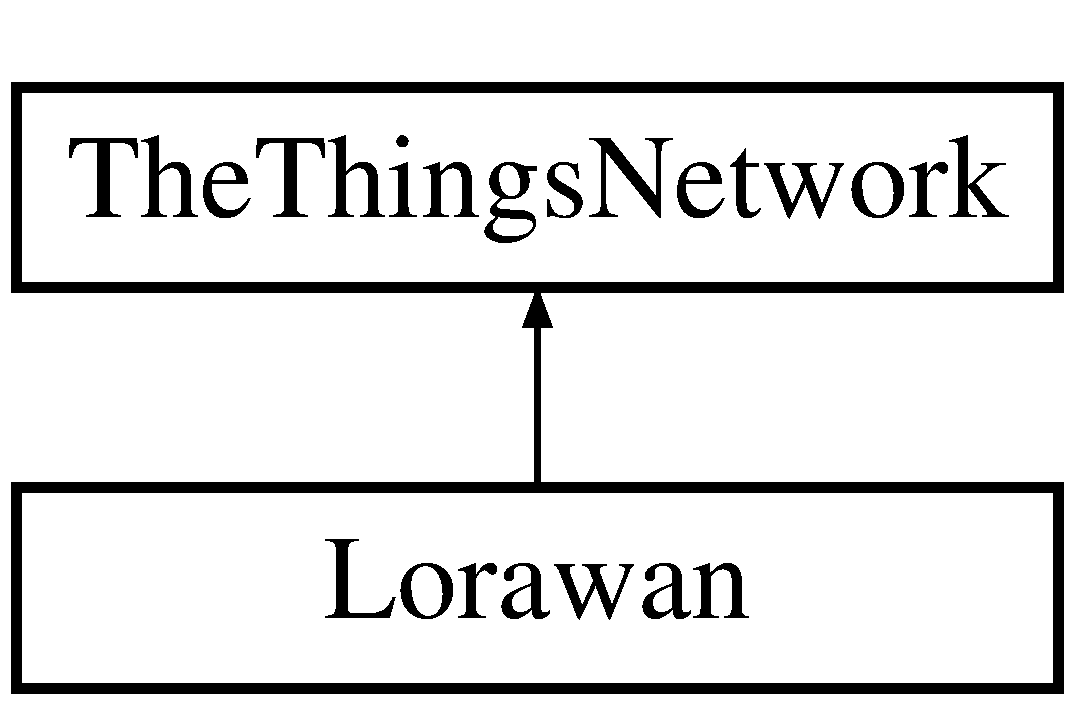
\includegraphics[height=2.000000cm]{class_lorawan}
\end{center}
\end{figure}
\subsection*{Public Member Functions}
\begin{DoxyCompactItemize}
\item 
\mbox{\hyperlink{class_lorawan_ad406457b082f8ae38594aa7daf632d1f}{Lorawan}} (Stream \&modem\+Stream, Stream \&debug\+Stream, ttn\+\_\+fp\+\_\+t fp, uint8\+\_\+t sf=T\+T\+N\+\_\+\+D\+E\+F\+A\+U\+L\+T\+\_\+\+SF, uint8\+\_\+t fsb=T\+T\+N\+\_\+\+D\+E\+F\+A\+U\+L\+T\+\_\+\+F\+SB)
\item 
bool \mbox{\hyperlink{class_lorawan_a590a79393a24359a9cc69bb133f72d56}{join}} ()
\item 
bool \mbox{\hyperlink{class_lorawan_ad8e01477e0f83ffd15a75309ee94ecc2}{provision}} ()
\item 
ttn\+\_\+response\+\_\+t \mbox{\hyperlink{class_lorawan_a0a82173d537813a749766aec6ae58fe8}{send\+Reading}} (int16\+\_\+t reading, uint8\+\_\+t power\+Level)
\item 
ttn\+\_\+response\+\_\+t \mbox{\hyperlink{class_lorawan_ae070b6740ad21efb2bd3355af0f49792}{send\+Still\+Alive}} (uint8\+\_\+t power\+Level)
\item 
ttn\+\_\+response\+\_\+t \mbox{\hyperlink{class_lorawan_acf1283d8a62ea919fec60a3634944576}{send\+Generic\+Error}} (uint8\+\_\+t power\+Level)
\item 
ttn\+\_\+response\+\_\+t \mbox{\hyperlink{class_lorawan_ac57100cd65b5f9f5aea4e0cd8c24dd12}{send\+Microcontroller\+Error}} (uint8\+\_\+t power\+Level)
\item 
ttn\+\_\+response\+\_\+t \mbox{\hyperlink{class_lorawan_a53f239940033d3a5630f4876911038f6}{send\+Sensor\+Error}} (uint8\+\_\+t power\+Level)
\item 
ttn\+\_\+response\+\_\+t \mbox{\hyperlink{class_lorawan_acf1ef0ac8ce453bccc0d08347af071f0}{send\+Battery\+Error}} (uint8\+\_\+t power\+Level)
\item 
ttn\+\_\+response\+\_\+t \mbox{\hyperlink{class_lorawan_a8d5565a2257a87ad9b39d78ea2ad38b8}{send\+Storage\+Error}} (uint8\+\_\+t power\+Level)
\item 
uint8\+\_\+t \mbox{\hyperlink{class_lorawan_ab24ea4c1ed2f9fdc6f64d9c0fe64ca60}{get\+Spread\+Factor}} ()
\item 
char $\ast$ \mbox{\hyperlink{class_lorawan_a2d454c9a1216a5ae80c3c20c6a3b5e32}{get\+Char\+App\+Eui}} ()
\item 
char $\ast$ \mbox{\hyperlink{class_lorawan_a2a95dfcf1dc5868cd6e8a5fb8c4e5231}{get\+App\+Key}} ()
\item 
void \mbox{\hyperlink{class_lorawan_a58ab6ca02b1c7e1f57618818ece5e86b}{set\+Spread\+Factor}} (uint8\+\_\+t spread\+Factor)
\item 
void \mbox{\hyperlink{class_lorawan_a0b79ba499200cd96859d518a47306fa9}{set\+Char\+App\+Eui}} (char $\ast$app\+Eui)
\item 
void \mbox{\hyperlink{class_lorawan_a0971c9c87d2a731bb5779953243a7016}{set\+App\+Key}} (char $\ast$app\+Key)
\end{DoxyCompactItemize}


\subsection{Detailed Description}
\mbox{\hyperlink{_lorawan_8h}{Lorawan.\+h}} -\/ Library for ultrasonic sensor water level measurements. Created by Natalie Mclaren, December 17, 2017. 

\subsection{Constructor \& Destructor Documentation}
\mbox{\Hypertarget{class_lorawan_ad406457b082f8ae38594aa7daf632d1f}\label{class_lorawan_ad406457b082f8ae38594aa7daf632d1f}} 
\index{Lorawan@{Lorawan}!Lorawan@{Lorawan}}
\index{Lorawan@{Lorawan}!Lorawan@{Lorawan}}
\subsubsection{\texorpdfstring{Lorawan()}{Lorawan()}}
{\footnotesize\ttfamily Lorawan\+::\+Lorawan (\begin{DoxyParamCaption}\item[{Stream \&}]{modem\+Stream,  }\item[{Stream \&}]{debug\+Stream,  }\item[{ttn\+\_\+fp\+\_\+t}]{fp,  }\item[{uint8\+\_\+t}]{sf = {\ttfamily TTN\+\_\+DEFAULT\+\_\+SF},  }\item[{uint8\+\_\+t}]{fsb = {\ttfamily TTN\+\_\+DEFAULT\+\_\+FSB} }\end{DoxyParamCaption})}

\mbox{\hyperlink{_lorawan_8cpp}{Lorawan.\+cpp}} -\/ Network based functions using lorawan Created by Natalie Mclaren, December 17, 2017. Constructor, including all other objects to be accessed. \mbox{\hyperlink{class_lorawan}{Lorawan}} functions joining/sending data to the network. 
\begin{DoxyParams}{Parameters}
{\em \{\+Stream\}} & \{\&moden\+Stream\} reference to Stream object. \\
\hline
{\em \{\+Stream\}} & \{\&debug\+Stream\} reference to Stream object. \\
\hline
{\em \{ttn\+\_\+fp\+\_\+t\}} & \{fp\} \\
\hline
{\em \{uint8\+\_\+t\}} & \{sf\} \mbox{\hyperlink{class_lorawan}{Lorawan}} spread factor \\
\hline
{\em \{uint8\+\_\+t\}} & \{fsb\} pointer to \mbox{\hyperlink{class_lorawan}{Lorawan}} object \\
\hline
\end{DoxyParams}
\begin{DoxyReturn}{Returns}
\{Void\} N/A 
\end{DoxyReturn}


\subsection{Member Function Documentation}
\mbox{\Hypertarget{class_lorawan_a2a95dfcf1dc5868cd6e8a5fb8c4e5231}\label{class_lorawan_a2a95dfcf1dc5868cd6e8a5fb8c4e5231}} 
\index{Lorawan@{Lorawan}!get\+App\+Key@{get\+App\+Key}}
\index{get\+App\+Key@{get\+App\+Key}!Lorawan@{Lorawan}}
\subsubsection{\texorpdfstring{get\+App\+Key()}{getAppKey()}}
{\footnotesize\ttfamily char $\ast$ Lorawan\+::get\+App\+Key (\begin{DoxyParamCaption}{ }\end{DoxyParamCaption})}

Getter to get the application\textquotesingle{}s key. 
\begin{DoxyParams}{Parameters}
{\em \{\+N/\+A\}} & \\
\hline
\end{DoxyParams}
\begin{DoxyReturn}{Returns}
\{char\} \{app\+Key\} The application key used 
\end{DoxyReturn}
\mbox{\Hypertarget{class_lorawan_a2d454c9a1216a5ae80c3c20c6a3b5e32}\label{class_lorawan_a2d454c9a1216a5ae80c3c20c6a3b5e32}} 
\index{Lorawan@{Lorawan}!get\+Char\+App\+Eui@{get\+Char\+App\+Eui}}
\index{get\+Char\+App\+Eui@{get\+Char\+App\+Eui}!Lorawan@{Lorawan}}
\subsubsection{\texorpdfstring{get\+Char\+App\+Eui()}{getCharAppEui()}}
{\footnotesize\ttfamily char $\ast$ Lorawan\+::get\+Char\+App\+Eui (\begin{DoxyParamCaption}{ }\end{DoxyParamCaption})}

Getter to get the application\textquotesingle{}s Eui. 
\begin{DoxyParams}{Parameters}
{\em \{\+N/\+A\}} & \\
\hline
\end{DoxyParams}
\begin{DoxyReturn}{Returns}
\{char\} \{app\+Eui\} The application Eui used 
\end{DoxyReturn}
\mbox{\Hypertarget{class_lorawan_ab24ea4c1ed2f9fdc6f64d9c0fe64ca60}\label{class_lorawan_ab24ea4c1ed2f9fdc6f64d9c0fe64ca60}} 
\index{Lorawan@{Lorawan}!get\+Spread\+Factor@{get\+Spread\+Factor}}
\index{get\+Spread\+Factor@{get\+Spread\+Factor}!Lorawan@{Lorawan}}
\subsubsection{\texorpdfstring{get\+Spread\+Factor()}{getSpreadFactor()}}
{\footnotesize\ttfamily uint8\+\_\+t Lorawan\+::get\+Spread\+Factor (\begin{DoxyParamCaption}{ }\end{DoxyParamCaption})}

Getter to get the \mbox{\hyperlink{class_lorawan}{Lorawan}} spread factor used. 
\begin{DoxyParams}{Parameters}
{\em \{\+N/\+A\}} & \\
\hline
\end{DoxyParams}
\begin{DoxyReturn}{Returns}
\{uint8\+\_\+t\} \{SF\} The spread factor. 
\end{DoxyReturn}
\mbox{\Hypertarget{class_lorawan_a590a79393a24359a9cc69bb133f72d56}\label{class_lorawan_a590a79393a24359a9cc69bb133f72d56}} 
\index{Lorawan@{Lorawan}!join@{join}}
\index{join@{join}!Lorawan@{Lorawan}}
\subsubsection{\texorpdfstring{join()}{join()}}
{\footnotesize\ttfamily bool Lorawan\+::join (\begin{DoxyParamCaption}{ }\end{DoxyParamCaption})}

Join the T\+TN. 
\begin{DoxyParams}{Parameters}
{\em N/A} & \\
\hline
\end{DoxyParams}
\begin{DoxyReturn}{Returns}
\{boolean\} True if it joined T\+TN, false if it didn\textquotesingle{}t 
\end{DoxyReturn}
\mbox{\Hypertarget{class_lorawan_ad8e01477e0f83ffd15a75309ee94ecc2}\label{class_lorawan_ad8e01477e0f83ffd15a75309ee94ecc2}} 
\index{Lorawan@{Lorawan}!provision@{provision}}
\index{provision@{provision}!Lorawan@{Lorawan}}
\subsubsection{\texorpdfstring{provision()}{provision()}}
{\footnotesize\ttfamily bool Lorawan\+::provision (\begin{DoxyParamCaption}{ }\end{DoxyParamCaption})}

Sets the information needed to activate the device. 
\begin{DoxyParams}{Parameters}
{\em \{char\}} & \{app\+Eui\} The application E\+UI \\
\hline
{\em \{char\}} & \{app\+Key\} The application key \\
\hline
\end{DoxyParams}
\begin{DoxyReturn}{Returns}
\{boolean\} True if successful, false otherwise 
\end{DoxyReturn}
\mbox{\Hypertarget{class_lorawan_acf1ef0ac8ce453bccc0d08347af071f0}\label{class_lorawan_acf1ef0ac8ce453bccc0d08347af071f0}} 
\index{Lorawan@{Lorawan}!send\+Battery\+Error@{send\+Battery\+Error}}
\index{send\+Battery\+Error@{send\+Battery\+Error}!Lorawan@{Lorawan}}
\subsubsection{\texorpdfstring{send\+Battery\+Error()}{sendBatteryError()}}
{\footnotesize\ttfamily ttn\+\_\+response\+\_\+t Lorawan\+::send\+Battery\+Error (\begin{DoxyParamCaption}\item[{uint8\+\_\+t}]{power\+Level }\end{DoxyParamCaption})}

Sends a Battery Error code. 
\begin{DoxyParams}{Parameters}
{\em \{uint8\+\_\+t\}} & \{power\+Level\} The processor\textquotesingle{}s battery power level \\
\hline
\end{DoxyParams}
\begin{DoxyReturn}{Returns}
\{ttn\+\_\+response\+\_\+t\} Returns a success or error code and logs the related error message i.\+e. \textquotesingle{}successful transmisson\textquotesingle{} 
\end{DoxyReturn}
\mbox{\Hypertarget{class_lorawan_acf1283d8a62ea919fec60a3634944576}\label{class_lorawan_acf1283d8a62ea919fec60a3634944576}} 
\index{Lorawan@{Lorawan}!send\+Generic\+Error@{send\+Generic\+Error}}
\index{send\+Generic\+Error@{send\+Generic\+Error}!Lorawan@{Lorawan}}
\subsubsection{\texorpdfstring{send\+Generic\+Error()}{sendGenericError()}}
{\footnotesize\ttfamily ttn\+\_\+response\+\_\+t Lorawan\+::send\+Generic\+Error (\begin{DoxyParamCaption}\item[{uint8\+\_\+t}]{power\+Level }\end{DoxyParamCaption})}

Sends a Generic Error code. 
\begin{DoxyParams}{Parameters}
{\em \{uint8\+\_\+t\}} & \{power\+Level\} The processor\textquotesingle{}s battery power level \\
\hline
\end{DoxyParams}
\begin{DoxyReturn}{Returns}
\{ttn\+\_\+response\+\_\+t\} Returns a success or error code and logs the related error message i.\+e. \textquotesingle{}successful transmisson\textquotesingle{} 
\end{DoxyReturn}
\mbox{\Hypertarget{class_lorawan_ac57100cd65b5f9f5aea4e0cd8c24dd12}\label{class_lorawan_ac57100cd65b5f9f5aea4e0cd8c24dd12}} 
\index{Lorawan@{Lorawan}!send\+Microcontroller\+Error@{send\+Microcontroller\+Error}}
\index{send\+Microcontroller\+Error@{send\+Microcontroller\+Error}!Lorawan@{Lorawan}}
\subsubsection{\texorpdfstring{send\+Microcontroller\+Error()}{sendMicrocontrollerError()}}
{\footnotesize\ttfamily ttn\+\_\+response\+\_\+t Lorawan\+::send\+Microcontroller\+Error (\begin{DoxyParamCaption}\item[{uint8\+\_\+t}]{power\+Level }\end{DoxyParamCaption})}

Sends a Microcontroller Error code. 
\begin{DoxyParams}{Parameters}
{\em \{uint8\+\_\+t\}} & \{power\+Level\} The processor\textquotesingle{}s battery power level \\
\hline
\end{DoxyParams}
\begin{DoxyReturn}{Returns}
\{ttn\+\_\+response\+\_\+t\} Returns a success or error code and logs the related error message i.\+e. \textquotesingle{}successful transmisson\textquotesingle{} 
\end{DoxyReturn}
\mbox{\Hypertarget{class_lorawan_a0a82173d537813a749766aec6ae58fe8}\label{class_lorawan_a0a82173d537813a749766aec6ae58fe8}} 
\index{Lorawan@{Lorawan}!send\+Reading@{send\+Reading}}
\index{send\+Reading@{send\+Reading}!Lorawan@{Lorawan}}
\subsubsection{\texorpdfstring{send\+Reading()}{sendReading()}}
{\footnotesize\ttfamily ttn\+\_\+response\+\_\+t Lorawan\+::send\+Reading (\begin{DoxyParamCaption}\item[{int16\+\_\+t}]{reading,  }\item[{uint8\+\_\+t}]{power\+Level }\end{DoxyParamCaption})}

Sends a reading. 
\begin{DoxyParams}{Parameters}
{\em \{int16\+\_\+t\}} & \{reading\} A reading from the sensor \\
\hline
{\em \{uint8\+\_\+t\}} & \{power\+Level\} The processor\textquotesingle{}s battery power level \\
\hline
\end{DoxyParams}
\begin{DoxyReturn}{Returns}
\{ttn\+\_\+response\+\_\+t\} Returns a success or error code and logs the related error message i.\+e. \textquotesingle{}successful transmisson\textquotesingle{} 
\end{DoxyReturn}
\mbox{\Hypertarget{class_lorawan_a53f239940033d3a5630f4876911038f6}\label{class_lorawan_a53f239940033d3a5630f4876911038f6}} 
\index{Lorawan@{Lorawan}!send\+Sensor\+Error@{send\+Sensor\+Error}}
\index{send\+Sensor\+Error@{send\+Sensor\+Error}!Lorawan@{Lorawan}}
\subsubsection{\texorpdfstring{send\+Sensor\+Error()}{sendSensorError()}}
{\footnotesize\ttfamily ttn\+\_\+response\+\_\+t Lorawan\+::send\+Sensor\+Error (\begin{DoxyParamCaption}\item[{uint8\+\_\+t}]{power\+Level }\end{DoxyParamCaption})}

Sends a \mbox{\hyperlink{class_sensor}{Sensor}} Error code. 
\begin{DoxyParams}{Parameters}
{\em \{uint8\+\_\+t\}} & \{power\+Level\} The processor\textquotesingle{}s battery power level \\
\hline
\end{DoxyParams}
\begin{DoxyReturn}{Returns}
\{ttn\+\_\+response\+\_\+t\} Returns a success or error code and logs the related error message i.\+e. \textquotesingle{}successful transmisson\textquotesingle{} 
\end{DoxyReturn}
\mbox{\Hypertarget{class_lorawan_ae070b6740ad21efb2bd3355af0f49792}\label{class_lorawan_ae070b6740ad21efb2bd3355af0f49792}} 
\index{Lorawan@{Lorawan}!send\+Still\+Alive@{send\+Still\+Alive}}
\index{send\+Still\+Alive@{send\+Still\+Alive}!Lorawan@{Lorawan}}
\subsubsection{\texorpdfstring{send\+Still\+Alive()}{sendStillAlive()}}
{\footnotesize\ttfamily ttn\+\_\+response\+\_\+t Lorawan\+::send\+Still\+Alive (\begin{DoxyParamCaption}\item[{uint8\+\_\+t}]{power\+Level }\end{DoxyParamCaption})}

Sends a \textquotesingle{}Still Here\textquotesingle{} code. 
\begin{DoxyParams}{Parameters}
{\em \{uint8\+\_\+t\}} & \{power\+Level\} The processor\textquotesingle{}s battery power level \\
\hline
\end{DoxyParams}
\begin{DoxyReturn}{Returns}
\{ttn\+\_\+response\+\_\+t\} Returns a success or error code and logs the related error message i.\+e. \textquotesingle{}successful transmisson\textquotesingle{} 
\end{DoxyReturn}
\mbox{\Hypertarget{class_lorawan_a8d5565a2257a87ad9b39d78ea2ad38b8}\label{class_lorawan_a8d5565a2257a87ad9b39d78ea2ad38b8}} 
\index{Lorawan@{Lorawan}!send\+Storage\+Error@{send\+Storage\+Error}}
\index{send\+Storage\+Error@{send\+Storage\+Error}!Lorawan@{Lorawan}}
\subsubsection{\texorpdfstring{send\+Storage\+Error()}{sendStorageError()}}
{\footnotesize\ttfamily ttn\+\_\+response\+\_\+t Lorawan\+::send\+Storage\+Error (\begin{DoxyParamCaption}\item[{uint8\+\_\+t}]{power\+Level }\end{DoxyParamCaption})}

Sends a Storage Error code. 
\begin{DoxyParams}{Parameters}
{\em \{uint8\+\_\+t\}} & \{power\+Level\} The processor\textquotesingle{}s battery power level \\
\hline
\end{DoxyParams}
\begin{DoxyReturn}{Returns}
\{ttn\+\_\+response\+\_\+t\} Returns a success or error code and logs the related error message i.\+e. \textquotesingle{}successful transmisson\textquotesingle{} 
\end{DoxyReturn}
\mbox{\Hypertarget{class_lorawan_a0971c9c87d2a731bb5779953243a7016}\label{class_lorawan_a0971c9c87d2a731bb5779953243a7016}} 
\index{Lorawan@{Lorawan}!set\+App\+Key@{set\+App\+Key}}
\index{set\+App\+Key@{set\+App\+Key}!Lorawan@{Lorawan}}
\subsubsection{\texorpdfstring{set\+App\+Key()}{setAppKey()}}
{\footnotesize\ttfamily void Lorawan\+::set\+App\+Key (\begin{DoxyParamCaption}\item[{char $\ast$}]{app\+Key }\end{DoxyParamCaption})}

Setter to set the applications key. 
\begin{DoxyParams}{Parameters}
{\em \{char\}} & \{app\+Key\} Pointer to the application\textquotesingle{}s key. \\
\hline
\end{DoxyParams}
\begin{DoxyReturn}{Returns}
\{Void\} 
\end{DoxyReturn}
\mbox{\Hypertarget{class_lorawan_a0b79ba499200cd96859d518a47306fa9}\label{class_lorawan_a0b79ba499200cd96859d518a47306fa9}} 
\index{Lorawan@{Lorawan}!set\+Char\+App\+Eui@{set\+Char\+App\+Eui}}
\index{set\+Char\+App\+Eui@{set\+Char\+App\+Eui}!Lorawan@{Lorawan}}
\subsubsection{\texorpdfstring{set\+Char\+App\+Eui()}{setCharAppEui()}}
{\footnotesize\ttfamily void Lorawan\+::set\+Char\+App\+Eui (\begin{DoxyParamCaption}\item[{char $\ast$}]{app\+Eui }\end{DoxyParamCaption})}

Setter to set the applications Eui. 
\begin{DoxyParams}{Parameters}
{\em \{char\}} & \{app\+Eui\} Pointer to the application\textquotesingle{}s Eui. \\
\hline
\end{DoxyParams}
\begin{DoxyReturn}{Returns}
\{Void\} 
\end{DoxyReturn}
\mbox{\Hypertarget{class_lorawan_a58ab6ca02b1c7e1f57618818ece5e86b}\label{class_lorawan_a58ab6ca02b1c7e1f57618818ece5e86b}} 
\index{Lorawan@{Lorawan}!set\+Spread\+Factor@{set\+Spread\+Factor}}
\index{set\+Spread\+Factor@{set\+Spread\+Factor}!Lorawan@{Lorawan}}
\subsubsection{\texorpdfstring{set\+Spread\+Factor()}{setSpreadFactor()}}
{\footnotesize\ttfamily void Lorawan\+::set\+Spread\+Factor (\begin{DoxyParamCaption}\item[{uint8\+\_\+t}]{spread\+Factor }\end{DoxyParamCaption})}

Setter to set the \mbox{\hyperlink{class_lorawan}{Lorawan}} spread factor used. 
\begin{DoxyParams}{Parameters}
{\em \{uint8\+\_\+t\}} & \{spread\+Factor\} The \mbox{\hyperlink{class_lorawan}{Lorawan}} spreadfactor \\
\hline
\end{DoxyParams}
\begin{DoxyReturn}{Returns}
\{Void\} 
\end{DoxyReturn}


The documentation for this class was generated from the following files\+:\begin{DoxyCompactItemize}
\item 
/\+Users/nataliemclaren/\+Documents/\+Uni/\+C\+O600/\+Flood-\/\+Sensor/\mbox{\hyperlink{_lorawan_8h}{Lorawan.\+h}}\item 
/\+Users/nataliemclaren/\+Documents/\+Uni/\+C\+O600/\+Flood-\/\+Sensor/\mbox{\hyperlink{_lorawan_8cpp}{Lorawan.\+cpp}}\end{DoxyCompactItemize}

\hypertarget{class_processor}{}\section{Processor Class Reference}
\label{class_processor}\index{Processor@{Processor}}


{\ttfamily \#include $<$Processor.\+h$>$}

\subsection*{Public Member Functions}
\begin{DoxyCompactItemize}
\item 
\mbox{\hyperlink{class_processor_a7f78050cf9700a4247df15a1eed5f88c}{Processor}} (\mbox{\hyperlink{class_sensor}{Sensor}} $\ast$sensor, \mbox{\hyperlink{class_s_d_card}{S\+D\+Card}} $\ast$sd\+Card, \mbox{\hyperlink{class_lorawan}{Lorawan}} $\ast$lorawan, byte interrput\+Pin, uint32\+\_\+t \mbox{\hyperlink{class_processor_a3d4df57c57607d2ed3ad9f2d4ff3e789}{delay\+Period}}=900000, uint32\+\_\+t delay\+Period\+A\+R\+Mode=600000, int16\+\_\+t A\+R\+Mode\+Activation\+Threshold=32000, int16\+\_\+t ignore\+Threshold=0)
\item 
void \mbox{\hyperlink{class_processor_a22e869ee49d974ad0ee7ee81961ab88f}{init}} ()
\item 
void \mbox{\hyperlink{class_processor_a694b889c3c6f8c09b998b4012d304d6e}{reading\+Process}} ()
\item 
void \mbox{\hyperlink{class_processor_a9316beb5903476939018dce45e992c53}{activate\+Or\+Deactivate\+A\+R\+Mode}} ()
\item 
void \mbox{\hyperlink{class_processor_a4b4e65040fd7bc17e978412c1af8e0c8}{adjust\+Ignore\+Threshold}} (int16\+\_\+t new\+Ignore\+Threshold)
\item 
void \mbox{\hyperlink{class_processor_a5b6762cf2679f4f47365aacb47b59ef5}{adjust\+A\+R\+Mode\+Delay}} (uint32\+\_\+t new\+Delay\+Period)
\item 
void \mbox{\hyperlink{class_processor_a58a2f6a482491cb003f4ff1bd45ba891}{adjust\+A\+R\+Mode\+Threshold}} (int16\+\_\+t new\+Activation\+Threshold)
\item 
void \mbox{\hyperlink{class_processor_a6ad79126a7694ed86f3f5ccc36b606bd}{delay\+With\+Period}} ()
\item 
void \mbox{\hyperlink{class_processor_a8759b7d9dc2d5f63fa9ca08f9211fd77}{change\+Measurement\+Period}} (uint32\+\_\+t milliseconds)
\item 
void \mbox{\hyperlink{class_processor_ae18acf2c55d0a3bcd7412f86d388808d}{recalibrate\+Sensor}} ()
\item 
void \mbox{\hyperlink{class_processor_a8083069e032fcd6e38c97cc31475200a}{trigger\+Clear\+Flash}} ()
\item 
void \mbox{\hyperlink{class_processor_a9e5c642ce356b8aebe5998158f31ded5}{adjust\+App\+Eui}} (String new\+App\+Eui)
\item 
void \mbox{\hyperlink{class_processor_adee07912124face3700bc988606b8f38}{adjust\+App\+Key}} (String new\+App\+Key)
\item 
float \mbox{\hyperlink{class_processor_aa467c82cb9a57d597487fc319c878c36}{get\+Battery\+Voltage}} ()
\item 
uint8\+\_\+t \mbox{\hyperlink{class_processor_ae2385e41f86895199fb37e524a3f1e86}{get\+Battery\+Voltage\+Byte}} ()
\item 
uint8\+\_\+t \mbox{\hyperlink{class_processor_a78b74d3be91182a263f77ff0f250408d}{get\+Estimated\+Power\+Level}} ()
\item 
void \mbox{\hyperlink{class_processor_aa60b755d3022b3b0f83f654e2b7e2e1d}{print\+Measurement\+To\+S\+D\+Log}} (int16\+\_\+t measurement)
\end{DoxyCompactItemize}
\subsection*{Public Attributes}
\begin{DoxyCompactItemize}
\item 
uint32\+\_\+t \mbox{\hyperlink{class_processor_a3d4df57c57607d2ed3ad9f2d4ff3e789}{delay\+Period}}
\item 
uint32\+\_\+t \mbox{\hyperlink{class_processor_acd8bba113bac81f4c5695cba7c9dd146}{measurement\+Period}}
\item 
bool \mbox{\hyperlink{class_processor_af51b6b3ce7074068195b5d3eb2442fdb}{A\+R\+Mode\+On}}
\end{DoxyCompactItemize}


\subsection{Detailed Description}
\mbox{\hyperlink{_processor_8h}{Processor.\+h}} -\/ Library for dealing with processor settings i.\+e. its engineering\+Menu\+Jumper/led pins. Created by Natalie Mclaren, December 18, 2017. 

\subsection{Constructor \& Destructor Documentation}
\mbox{\Hypertarget{class_processor_a7f78050cf9700a4247df15a1eed5f88c}\label{class_processor_a7f78050cf9700a4247df15a1eed5f88c}} 
\index{Processor@{Processor}!Processor@{Processor}}
\index{Processor@{Processor}!Processor@{Processor}}
\subsubsection{\texorpdfstring{Processor()}{Processor()}}
{\footnotesize\ttfamily Processor\+::\+Processor (\begin{DoxyParamCaption}\item[{\mbox{\hyperlink{class_sensor}{Sensor}} $\ast$}]{sensor,  }\item[{\mbox{\hyperlink{class_s_d_card}{S\+D\+Card}} $\ast$}]{sd\+Card,  }\item[{\mbox{\hyperlink{class_lorawan}{Lorawan}} $\ast$}]{lorawan,  }\item[{byte}]{engineering\+Menu\+Jumper\+Pin,  }\item[{uint32\+\_\+t}]{delay\+Period = {\ttfamily 900000},  }\item[{uint32\+\_\+t}]{delay\+Period\+A\+R\+Mode = {\ttfamily 600000},  }\item[{int16\+\_\+t}]{A\+R\+Mode\+Activation\+Threshold = {\ttfamily 32000},  }\item[{int16\+\_\+t}]{ignore\+Threshold = {\ttfamily 0} }\end{DoxyParamCaption})}

\mbox{\hyperlink{class_processor}{Processor}} constructor Sets default device settings values (delay\+Period etc...) 
\begin{DoxyParams}{Parameters}
{\em \{\+Sensor\}} & \{$\ast$sensor\} pointer to \mbox{\hyperlink{class_sensor}{Sensor}} object. \\
\hline
{\em \{\+S\+D\+Card\}} & \{$\ast$sd\+Card\} pointer to \mbox{\hyperlink{class_s_d_card}{S\+D\+Card}} object. \\
\hline
{\em \{\+Lorawan\}} & \{$\ast$lorawan\} pointer to \mbox{\hyperlink{class_lorawan}{Lorawan}} object. \\
\hline
{\em \{byte\}} & \{engineering\+Menu\+Jumper\+Pin\} engineering menu button interrupt pin number \\
\hline
{\em \{uint32\+\_\+t\}} & \{delay\+Period\} the delay period value between each samples \\
\hline
{\em \{uint32\+\_\+t\}} & \{delay\+Period\+A\+R\+Mode\} the accelerated reading mode value (less of a delay than the delay period) \\
\hline
{\em \{int16\+\_\+t\}} & \{A\+R\+Mode\+Activation\+Threshold\} the threshold which activates the A\+R\+Mode \\
\hline
{\em \{int16\+\_\+t\}} & \{ignore\+Threshold\} threshold (mm) for which the sensor should ignore readings -\/ don\textquotesingle{}t send any info to server \\
\hline
\end{DoxyParams}
\begin{DoxyReturn}{Returns}
N/A 
\end{DoxyReturn}


\subsection{Member Function Documentation}
\mbox{\Hypertarget{class_processor_a9316beb5903476939018dce45e992c53}\label{class_processor_a9316beb5903476939018dce45e992c53}} 
\index{Processor@{Processor}!activate\+Or\+Deactivate\+A\+R\+Mode@{activate\+Or\+Deactivate\+A\+R\+Mode}}
\index{activate\+Or\+Deactivate\+A\+R\+Mode@{activate\+Or\+Deactivate\+A\+R\+Mode}!Processor@{Processor}}
\subsubsection{\texorpdfstring{activate\+Or\+Deactivate\+A\+R\+Mode()}{activateOrDeactivateARMode()}}
{\footnotesize\ttfamily void Processor\+::activate\+Or\+Deactivate\+A\+R\+Mode (\begin{DoxyParamCaption}{ }\end{DoxyParamCaption})}

Swaps delay\+Period and delay\+Period\+A\+R\+Mode variables to activate/deactivate Accelerated Readings mode. 
\begin{DoxyParams}{Parameters}
{\em N/A} & \\
\hline
\end{DoxyParams}
\begin{DoxyReturn}{Returns}
\{void\} N/A 
\end{DoxyReturn}
\mbox{\Hypertarget{class_processor_a9e5c642ce356b8aebe5998158f31ded5}\label{class_processor_a9e5c642ce356b8aebe5998158f31ded5}} 
\index{Processor@{Processor}!adjust\+App\+Eui@{adjust\+App\+Eui}}
\index{adjust\+App\+Eui@{adjust\+App\+Eui}!Processor@{Processor}}
\subsubsection{\texorpdfstring{adjust\+App\+Eui()}{adjustAppEui()}}
{\footnotesize\ttfamily void Processor\+::adjust\+App\+Eui (\begin{DoxyParamCaption}\item[{String}]{new\+App\+Eui }\end{DoxyParamCaption})}

Adjust the application\textquotesingle{}s Eui 
\begin{DoxyParams}{Parameters}
{\em \{\+String\}} & \{new\+App\+Eui\} The new Eui value \\
\hline
\end{DoxyParams}
\begin{DoxyReturn}{Returns}
\{N/A\} 
\end{DoxyReturn}
\mbox{\Hypertarget{class_processor_adee07912124face3700bc988606b8f38}\label{class_processor_adee07912124face3700bc988606b8f38}} 
\index{Processor@{Processor}!adjust\+App\+Key@{adjust\+App\+Key}}
\index{adjust\+App\+Key@{adjust\+App\+Key}!Processor@{Processor}}
\subsubsection{\texorpdfstring{adjust\+App\+Key()}{adjustAppKey()}}
{\footnotesize\ttfamily void Processor\+::adjust\+App\+Key (\begin{DoxyParamCaption}\item[{String}]{new\+App\+Key }\end{DoxyParamCaption})}

Adjust the application\textquotesingle{}s key 
\begin{DoxyParams}{Parameters}
{\em \{\+String\}} & \{new\+App\+Key\} The new application key value \\
\hline
\end{DoxyParams}
\begin{DoxyReturn}{Returns}
\{N/A\} 
\end{DoxyReturn}
\mbox{\Hypertarget{class_processor_a5b6762cf2679f4f47365aacb47b59ef5}\label{class_processor_a5b6762cf2679f4f47365aacb47b59ef5}} 
\index{Processor@{Processor}!adjust\+A\+R\+Mode\+Delay@{adjust\+A\+R\+Mode\+Delay}}
\index{adjust\+A\+R\+Mode\+Delay@{adjust\+A\+R\+Mode\+Delay}!Processor@{Processor}}
\subsubsection{\texorpdfstring{adjust\+A\+R\+Mode\+Delay()}{adjustARModeDelay()}}
{\footnotesize\ttfamily void Processor\+::adjust\+A\+R\+Mode\+Delay (\begin{DoxyParamCaption}\item[{uint32\+\_\+t}]{new\+Delay\+Period }\end{DoxyParamCaption})}

Set delay period to be used whilst the device is in AR (Accelerated Readings) Mode. 
\begin{DoxyParams}{Parameters}
{\em \{uint32\+\_\+t\}} & \{new\+Delay\+Period\} new delay period to be used. \\
\hline
\end{DoxyParams}
\begin{DoxyReturn}{Returns}
\{void\} N/A 
\end{DoxyReturn}
\mbox{\Hypertarget{class_processor_a58a2f6a482491cb003f4ff1bd45ba891}\label{class_processor_a58a2f6a482491cb003f4ff1bd45ba891}} 
\index{Processor@{Processor}!adjust\+A\+R\+Mode\+Threshold@{adjust\+A\+R\+Mode\+Threshold}}
\index{adjust\+A\+R\+Mode\+Threshold@{adjust\+A\+R\+Mode\+Threshold}!Processor@{Processor}}
\subsubsection{\texorpdfstring{adjust\+A\+R\+Mode\+Threshold()}{adjustARModeThreshold()}}
{\footnotesize\ttfamily void Processor\+::adjust\+A\+R\+Mode\+Threshold (\begin{DoxyParamCaption}\item[{int16\+\_\+t}]{new\+Activation\+Threshold }\end{DoxyParamCaption})}

Set max river depth threshold to trigger AR Mode (Measured in\+: mm). 
\begin{DoxyParams}{Parameters}
{\em \{int16\+\_\+t\}} & \{new\+Activation\+Threshold\} new maximum threshold to trigger AR mode. \\
\hline
\end{DoxyParams}
\begin{DoxyReturn}{Returns}
\{void\} N/A 
\end{DoxyReturn}
\mbox{\Hypertarget{class_processor_a4b4e65040fd7bc17e978412c1af8e0c8}\label{class_processor_a4b4e65040fd7bc17e978412c1af8e0c8}} 
\index{Processor@{Processor}!adjust\+Ignore\+Threshold@{adjust\+Ignore\+Threshold}}
\index{adjust\+Ignore\+Threshold@{adjust\+Ignore\+Threshold}!Processor@{Processor}}
\subsubsection{\texorpdfstring{adjust\+Ignore\+Threshold()}{adjustIgnoreThreshold()}}
{\footnotesize\ttfamily void Processor\+::adjust\+Ignore\+Threshold (\begin{DoxyParamCaption}\item[{int16\+\_\+t}]{new\+Ignore\+Threshold }\end{DoxyParamCaption})}

Set minimum river depth threshold (anything below this value will be ignored, and considered \char`\"{}not worth\char`\"{} sending) (mm). 
\begin{DoxyParams}{Parameters}
{\em \{int16\+\_\+t\}} & \{new\+Ignore\+Threshold\} new minimum river depth threshold to be set (mm). \\
\hline
\end{DoxyParams}
\begin{DoxyReturn}{Returns}
\{void\} N/A 
\end{DoxyReturn}
\mbox{\Hypertarget{class_processor_a8759b7d9dc2d5f63fa9ca08f9211fd77}\label{class_processor_a8759b7d9dc2d5f63fa9ca08f9211fd77}} 
\index{Processor@{Processor}!change\+Measurement\+Period@{change\+Measurement\+Period}}
\index{change\+Measurement\+Period@{change\+Measurement\+Period}!Processor@{Processor}}
\subsubsection{\texorpdfstring{change\+Measurement\+Period()}{changeMeasurementPeriod()}}
{\footnotesize\ttfamily void Processor\+::change\+Measurement\+Period (\begin{DoxyParamCaption}\item[{uint32\+\_\+t}]{milliseconds }\end{DoxyParamCaption})}

Set the delay period between each measurement to be taken. 
\begin{DoxyParams}{Parameters}
{\em \{uint32\+\_\+t\}} & \{minutes\} new delay period (in minutes) set. \\
\hline
\end{DoxyParams}
\begin{DoxyReturn}{Returns}
\{void\} N/A 
\end{DoxyReturn}
\mbox{\Hypertarget{class_processor_a6ad79126a7694ed86f3f5ccc36b606bd}\label{class_processor_a6ad79126a7694ed86f3f5ccc36b606bd}} 
\index{Processor@{Processor}!delay\+With\+Period@{delay\+With\+Period}}
\index{delay\+With\+Period@{delay\+With\+Period}!Processor@{Processor}}
\subsubsection{\texorpdfstring{delay\+With\+Period()}{delayWithPeriod()}}
{\footnotesize\ttfamily void Processor\+::delay\+With\+Period (\begin{DoxyParamCaption}{ }\end{DoxyParamCaption})}

Makes the entire device sleep for a specified period of time. Used to sleep in between taking river depth measurements. 
\begin{DoxyParams}{Parameters}
{\em N/A} & \\
\hline
\end{DoxyParams}
\begin{DoxyReturn}{Returns}
\{void\} N/A 
\end{DoxyReturn}
\mbox{\Hypertarget{class_processor_aa467c82cb9a57d597487fc319c878c36}\label{class_processor_aa467c82cb9a57d597487fc319c878c36}} 
\index{Processor@{Processor}!get\+Battery\+Voltage@{get\+Battery\+Voltage}}
\index{get\+Battery\+Voltage@{get\+Battery\+Voltage}!Processor@{Processor}}
\subsubsection{\texorpdfstring{get\+Battery\+Voltage()}{getBatteryVoltage()}}
{\footnotesize\ttfamily float Processor\+::get\+Battery\+Voltage (\begin{DoxyParamCaption}{ }\end{DoxyParamCaption})}

Calculates and returns current battery voltage value. Gets an average of 5 readings over 5 seconds. 
\begin{DoxyParams}{Parameters}
{\em N/A} & \\
\hline
\end{DoxyParams}
\begin{DoxyReturn}{Returns}
\{float\} returns measuredvbat value. 
\end{DoxyReturn}
\mbox{\Hypertarget{class_processor_ae2385e41f86895199fb37e524a3f1e86}\label{class_processor_ae2385e41f86895199fb37e524a3f1e86}} 
\index{Processor@{Processor}!get\+Battery\+Voltage\+Byte@{get\+Battery\+Voltage\+Byte}}
\index{get\+Battery\+Voltage\+Byte@{get\+Battery\+Voltage\+Byte}!Processor@{Processor}}
\subsubsection{\texorpdfstring{get\+Battery\+Voltage\+Byte()}{getBatteryVoltageByte()}}
{\footnotesize\ttfamily uint8\+\_\+t Processor\+::get\+Battery\+Voltage\+Byte (\begin{DoxyParamCaption}{ }\end{DoxyParamCaption})}

Converts battery voltage to a byte to be sent to the A\+PI. Done to save T\+TN bandwidth (So we don\textquotesingle{}t need to send send a full floating point number). 
\begin{DoxyParams}{Parameters}
{\em N/A} & \\
\hline
\end{DoxyParams}
\begin{DoxyReturn}{Returns}
\{uint8\+\_\+t\} returns voltage as an interger between 1 and 100 to be then recalculated in the A\+PI 
\end{DoxyReturn}
\mbox{\Hypertarget{class_processor_a78b74d3be91182a263f77ff0f250408d}\label{class_processor_a78b74d3be91182a263f77ff0f250408d}} 
\index{Processor@{Processor}!get\+Estimated\+Power\+Level@{get\+Estimated\+Power\+Level}}
\index{get\+Estimated\+Power\+Level@{get\+Estimated\+Power\+Level}!Processor@{Processor}}
\subsubsection{\texorpdfstring{get\+Estimated\+Power\+Level()}{getEstimatedPowerLevel()}}
{\footnotesize\ttfamily uint8\+\_\+t Processor\+::get\+Estimated\+Power\+Level (\begin{DoxyParamCaption}{ }\end{DoxyParamCaption})}

Calculates and returns estimated battery percentage (powerlevel/capacity) based on voltage and m\+Ah of the battery. Expected default battery\+: 4.\+2v max (and 3.\+2v min cut off) 700m\+Ah 
\begin{DoxyParams}{Parameters}
{\em N/A} & \\
\hline
\end{DoxyParams}
\begin{DoxyReturn}{Returns}
\{uint8\+\_\+t\} return battery percentage. 
\end{DoxyReturn}
\mbox{\Hypertarget{class_processor_a22e869ee49d974ad0ee7ee81961ab88f}\label{class_processor_a22e869ee49d974ad0ee7ee81961ab88f}} 
\index{Processor@{Processor}!init@{init}}
\index{init@{init}!Processor@{Processor}}
\subsubsection{\texorpdfstring{init()}{init()}}
{\footnotesize\ttfamily void Processor\+::init (\begin{DoxyParamCaption}{ }\end{DoxyParamCaption})}

Initialise default sensor settings and values Takes initial river depth input from engineer user from serial input to populate other defaults. 
\begin{DoxyParams}{Parameters}
{\em N/A} & \\
\hline
\end{DoxyParams}
\begin{DoxyReturn}{Returns}
\{void\} N/A 
\end{DoxyReturn}
\mbox{\Hypertarget{class_processor_aa60b755d3022b3b0f83f654e2b7e2e1d}\label{class_processor_aa60b755d3022b3b0f83f654e2b7e2e1d}} 
\index{Processor@{Processor}!print\+Measurement\+To\+S\+D\+Log@{print\+Measurement\+To\+S\+D\+Log}}
\index{print\+Measurement\+To\+S\+D\+Log@{print\+Measurement\+To\+S\+D\+Log}!Processor@{Processor}}
\subsubsection{\texorpdfstring{print\+Measurement\+To\+S\+D\+Log()}{printMeasurementToSDLog()}}
{\footnotesize\ttfamily void Processor\+::print\+Measurement\+To\+S\+D\+Log (\begin{DoxyParamCaption}\item[{int16\+\_\+t}]{measurement }\end{DoxyParamCaption})}

Call \mbox{\hyperlink{class_s_d_card}{S\+D\+Card}} class function to store the last measurement sent to a log on the SD card. 
\begin{DoxyParams}{Parameters}
{\em \{int16\+\_\+t\}} & \{last\+Measurement\+Sent\} last measurement that was sent to the api sucessfully. \\
\hline
\end{DoxyParams}
\begin{DoxyReturn}{Returns}
\{void\} N/A 
\end{DoxyReturn}
\mbox{\Hypertarget{class_processor_a694b889c3c6f8c09b998b4012d304d6e}\label{class_processor_a694b889c3c6f8c09b998b4012d304d6e}} 
\index{Processor@{Processor}!reading\+Process@{reading\+Process}}
\index{reading\+Process@{reading\+Process}!Processor@{Processor}}
\subsubsection{\texorpdfstring{reading\+Process()}{readingProcess()}}
{\footnotesize\ttfamily void Processor\+::reading\+Process (\begin{DoxyParamCaption}{ }\end{DoxyParamCaption})}

Process current river depth measurement, and send if relevant. 
\begin{DoxyParams}{Parameters}
{\em N/A} & \\
\hline
\end{DoxyParams}
\begin{DoxyReturn}{Returns}
\{void\} N/A 
\end{DoxyReturn}
\mbox{\Hypertarget{class_processor_ae18acf2c55d0a3bcd7412f86d388808d}\label{class_processor_ae18acf2c55d0a3bcd7412f86d388808d}} 
\index{Processor@{Processor}!recalibrate\+Sensor@{recalibrate\+Sensor}}
\index{recalibrate\+Sensor@{recalibrate\+Sensor}!Processor@{Processor}}
\subsubsection{\texorpdfstring{recalibrate\+Sensor()}{recalibrateSensor()}}
{\footnotesize\ttfamily void Processor\+::recalibrate\+Sensor (\begin{DoxyParamCaption}{ }\end{DoxyParamCaption})}

Used to calibrate the sensor as done in initial setup. Allows the engineer to input an initial depth for the river, for which the distance from sensor to river bed can be calculated.


\begin{DoxyParams}{Parameters}
{\em \{\+N/\+A\}} & \\
\hline
\end{DoxyParams}
\begin{DoxyReturn}{Returns}
\{N/A\} 
\end{DoxyReturn}
\mbox{\Hypertarget{class_processor_a8083069e032fcd6e38c97cc31475200a}\label{class_processor_a8083069e032fcd6e38c97cc31475200a}} 
\index{Processor@{Processor}!trigger\+Clear\+Flash@{trigger\+Clear\+Flash}}
\index{trigger\+Clear\+Flash@{trigger\+Clear\+Flash}!Processor@{Processor}}
\subsubsection{\texorpdfstring{trigger\+Clear\+Flash()}{triggerClearFlash()}}
{\footnotesize\ttfamily void Processor\+::trigger\+Clear\+Flash (\begin{DoxyParamCaption}{ }\end{DoxyParamCaption})}

Clear the device settings variables stored in the flash storage. 
\begin{DoxyParams}{Parameters}
{\em \{\+N/\+A\}} & \\
\hline
\end{DoxyParams}
\begin{DoxyReturn}{Returns}
\{Void\} 
\end{DoxyReturn}


\subsection{Member Data Documentation}
\mbox{\Hypertarget{class_processor_af51b6b3ce7074068195b5d3eb2442fdb}\label{class_processor_af51b6b3ce7074068195b5d3eb2442fdb}} 
\index{Processor@{Processor}!A\+R\+Mode\+On@{A\+R\+Mode\+On}}
\index{A\+R\+Mode\+On@{A\+R\+Mode\+On}!Processor@{Processor}}
\subsubsection{\texorpdfstring{A\+R\+Mode\+On}{ARModeOn}}
{\footnotesize\ttfamily bool Processor\+::\+A\+R\+Mode\+On}

\mbox{\Hypertarget{class_processor_a3d4df57c57607d2ed3ad9f2d4ff3e789}\label{class_processor_a3d4df57c57607d2ed3ad9f2d4ff3e789}} 
\index{Processor@{Processor}!delay\+Period@{delay\+Period}}
\index{delay\+Period@{delay\+Period}!Processor@{Processor}}
\subsubsection{\texorpdfstring{delay\+Period}{delayPeriod}}
{\footnotesize\ttfamily uint32\+\_\+t Processor\+::delay\+Period}

\mbox{\Hypertarget{class_processor_acd8bba113bac81f4c5695cba7c9dd146}\label{class_processor_acd8bba113bac81f4c5695cba7c9dd146}} 
\index{Processor@{Processor}!measurement\+Period@{measurement\+Period}}
\index{measurement\+Period@{measurement\+Period}!Processor@{Processor}}
\subsubsection{\texorpdfstring{measurement\+Period}{measurementPeriod}}
{\footnotesize\ttfamily uint32\+\_\+t Processor\+::measurement\+Period}



The documentation for this class was generated from the following files\+:\begin{DoxyCompactItemize}
\item 
/\+Users/nataliemclaren/\+Documents/\+Uni/\+C\+O600/\+Flood-\/\+Sensor/\mbox{\hyperlink{_processor_8h}{Processor.\+h}}\item 
/\+Users/nataliemclaren/\+Documents/\+Uni/\+C\+O600/\+Flood-\/\+Sensor/\mbox{\hyperlink{_processor_8cpp}{Processor.\+cpp}}\end{DoxyCompactItemize}

\hypertarget{class_s_d_card}{}\section{S\+D\+Card Class Reference}
\label{class_s_d_card}\index{S\+D\+Card@{S\+D\+Card}}


{\ttfamily \#include $<$S\+D\+Card.\+h$>$}

\subsection*{Public Member Functions}
\begin{DoxyCompactItemize}
\item 
\mbox{\hyperlink{class_s_d_card_aa57f64cf28817d210706222f60be9001}{S\+D\+Card}} ()
\item 
bool \mbox{\hyperlink{class_s_d_card_a7d5b2551a395d7bf883f425fb98b0b0d}{init}} ()
\item 
void \mbox{\hyperlink{class_s_d_card_a62c472309bd91560a29430d6946c05fb}{check\+Card\+Memory}} ()
\item 
bool \mbox{\hyperlink{class_s_d_card_ab43bfe585365622d71e30194a404125c}{file\+Has\+Reached\+Size\+Limit}} ()
\item 
bool \mbox{\hyperlink{class_s_d_card_a9c0edb3dd7e157501776d9760705a757}{read\+Log}} ()
\item 
bool \mbox{\hyperlink{class_s_d_card_ad5832b1d4274a99ca975f4c570584f53}{test\+Read\+Log}} (String data)
\item 
bool \mbox{\hyperlink{class_s_d_card_aa65251052d32bcaff9f087080118525f}{write\+To\+Log}} (String data)
\end{DoxyCompactItemize}
\subsection*{Public Attributes}
\begin{DoxyCompactItemize}
\item 
File \mbox{\hyperlink{class_s_d_card_a2e9756d5c5478bee2d7977a0c66ec47f}{my\+File}}
\item 
Sd\+Volume \mbox{\hyperlink{class_s_d_card_a143b4a79b09f0c1d6d71155b51dfefcb}{volume}}
\item 
Sd\+File \mbox{\hyperlink{class_s_d_card_a6e02af8a10a45955da7c560ea148ca4d}{root}}
\item 
Sd2\+Card \mbox{\hyperlink{class_s_d_card_a20919e15549972b09ad3c063c35fcf59}{card}}
\item 
uint32\+\_\+t \mbox{\hyperlink{class_s_d_card_a9f97edfb78131f459dbbda495903663e}{file\+Size}}
\end{DoxyCompactItemize}


\subsection{Detailed Description}
\mbox{\hyperlink{_s_d_card_8h}{S\+D\+Card.\+h}} -\/ Library for dealing with writing/retrieving data to/from \mbox{\hyperlink{class_s_d_card}{S\+D\+Card}}. Created by Natalie Mclaren, December 17, 2017. 

\subsection{Constructor \& Destructor Documentation}
\mbox{\Hypertarget{class_s_d_card_aa57f64cf28817d210706222f60be9001}\label{class_s_d_card_aa57f64cf28817d210706222f60be9001}} 
\index{S\+D\+Card@{S\+D\+Card}!S\+D\+Card@{S\+D\+Card}}
\index{S\+D\+Card@{S\+D\+Card}!S\+D\+Card@{S\+D\+Card}}
\subsubsection{\texorpdfstring{S\+D\+Card()}{SDCard()}}
{\footnotesize\ttfamily S\+D\+Card\+::\+S\+D\+Card (\begin{DoxyParamCaption}{ }\end{DoxyParamCaption})}

\mbox{\hyperlink{class_s_d_card}{S\+D\+Card}} constructor 
\begin{DoxyParams}{Parameters}
{\em N/A} & \\
\hline
\end{DoxyParams}
\begin{DoxyReturn}{Returns}
N/A 
\end{DoxyReturn}


\subsection{Member Function Documentation}
\mbox{\Hypertarget{class_s_d_card_a62c472309bd91560a29430d6946c05fb}\label{class_s_d_card_a62c472309bd91560a29430d6946c05fb}} 
\index{S\+D\+Card@{S\+D\+Card}!check\+Card\+Memory@{check\+Card\+Memory}}
\index{check\+Card\+Memory@{check\+Card\+Memory}!S\+D\+Card@{S\+D\+Card}}
\subsubsection{\texorpdfstring{check\+Card\+Memory()}{checkCardMemory()}}
{\footnotesize\ttfamily void S\+D\+Card\+::check\+Card\+Memory (\begin{DoxyParamCaption}{ }\end{DoxyParamCaption})}

Print details of SD card -\/ memory available, F\+AT type etc Debugging function to check the contents of the SD card. 
\begin{DoxyParams}{Parameters}
{\em N/A} & \\
\hline
\end{DoxyParams}
\begin{DoxyReturn}{Returns}
\{void\} N/A 
\end{DoxyReturn}
\mbox{\Hypertarget{class_s_d_card_ab43bfe585365622d71e30194a404125c}\label{class_s_d_card_ab43bfe585365622d71e30194a404125c}} 
\index{S\+D\+Card@{S\+D\+Card}!file\+Has\+Reached\+Size\+Limit@{file\+Has\+Reached\+Size\+Limit}}
\index{file\+Has\+Reached\+Size\+Limit@{file\+Has\+Reached\+Size\+Limit}!S\+D\+Card@{S\+D\+Card}}
\subsubsection{\texorpdfstring{file\+Has\+Reached\+Size\+Limit()}{fileHasReachedSizeLimit()}}
{\footnotesize\ttfamily bool S\+D\+Card\+::file\+Has\+Reached\+Size\+Limit (\begin{DoxyParamCaption}{ }\end{DoxyParamCaption})}

Check whether the text file is about to reach its size limit (7741678351 bytes or just under 7.\+21 GB) 
\begin{DoxyParams}{Parameters}
{\em N/A} & \\
\hline
\end{DoxyParams}
\begin{DoxyReturn}{Returns}
\{bool\} True if the text file is about to reach its size limit. False otherwise. 
\end{DoxyReturn}
\mbox{\Hypertarget{class_s_d_card_a7d5b2551a395d7bf883f425fb98b0b0d}\label{class_s_d_card_a7d5b2551a395d7bf883f425fb98b0b0d}} 
\index{S\+D\+Card@{S\+D\+Card}!init@{init}}
\index{init@{init}!S\+D\+Card@{S\+D\+Card}}
\subsubsection{\texorpdfstring{init()}{init()}}
{\footnotesize\ttfamily bool S\+D\+Card\+::init (\begin{DoxyParamCaption}{ }\end{DoxyParamCaption})}

During setup, this function initialises the SD Card and its library, and reads the card\textquotesingle{}s file size to store in a class variable. 
\begin{DoxyParams}{Parameters}
{\em N/A} & \\
\hline
\end{DoxyParams}
\begin{DoxyReturn}{Returns}
\{bool\} True if the text file was successfully opened for reading. False otherwise. 
\end{DoxyReturn}
\mbox{\Hypertarget{class_s_d_card_a9c0edb3dd7e157501776d9760705a757}\label{class_s_d_card_a9c0edb3dd7e157501776d9760705a757}} 
\index{S\+D\+Card@{S\+D\+Card}!read\+Log@{read\+Log}}
\index{read\+Log@{read\+Log}!S\+D\+Card@{S\+D\+Card}}
\subsubsection{\texorpdfstring{read\+Log()}{readLog()}}
{\footnotesize\ttfamily bool S\+D\+Card\+::read\+Log (\begin{DoxyParamCaption}{ }\end{DoxyParamCaption})}

Read the contents of the SD Card text file. 
\begin{DoxyParams}{Parameters}
{\em N/A} & \\
\hline
\end{DoxyParams}
\begin{DoxyReturn}{Returns}
\{bool\} True if the file was successfully opened for readings, false otherwise. 
\end{DoxyReturn}
\mbox{\Hypertarget{class_s_d_card_ad5832b1d4274a99ca975f4c570584f53}\label{class_s_d_card_ad5832b1d4274a99ca975f4c570584f53}} 
\index{S\+D\+Card@{S\+D\+Card}!test\+Read\+Log@{test\+Read\+Log}}
\index{test\+Read\+Log@{test\+Read\+Log}!S\+D\+Card@{S\+D\+Card}}
\subsubsection{\texorpdfstring{test\+Read\+Log()}{testReadLog()}}
{\footnotesize\ttfamily bool S\+D\+Card\+::test\+Read\+Log (\begin{DoxyParamCaption}\item[{String}]{test\+String }\end{DoxyParamCaption})}

Used to test that the last written value in the SD Card text file can be read. It finds the last value in the text file and compares it to the test string. They should equal the same, as the same test string is called in the write log function prior to this function call during the engineering menu test. 
\begin{DoxyParams}{Parameters}
{\em \{\+String\}} & \{test\+String\} \\
\hline
\end{DoxyParams}
\begin{DoxyReturn}{Returns}
\{bool\} True if the last value read from the text file matches the test string. False otherwise. 
\end{DoxyReturn}
\mbox{\Hypertarget{class_s_d_card_aa65251052d32bcaff9f087080118525f}\label{class_s_d_card_aa65251052d32bcaff9f087080118525f}} 
\index{S\+D\+Card@{S\+D\+Card}!write\+To\+Log@{write\+To\+Log}}
\index{write\+To\+Log@{write\+To\+Log}!S\+D\+Card@{S\+D\+Card}}
\subsubsection{\texorpdfstring{write\+To\+Log()}{writeToLog()}}
{\footnotesize\ttfamily bool S\+D\+Card\+::write\+To\+Log (\begin{DoxyParamCaption}\item[{String}]{last\+Measurement\+Sent }\end{DoxyParamCaption})}

Print the last measurement sent onto a new line in the SD Card text file. 
\begin{DoxyParams}{Parameters}
{\em \{\+String\}} & \{last\+Measurement\+Sent\} last measurement value sent successfully, to be logged. \\
\hline
\end{DoxyParams}
\begin{DoxyReturn}{Returns}
\{bool\} True if the last\+Measurement\+Sent was successfully written to the text file. False if it fails to write or if the text file failed to open. 
\end{DoxyReturn}


\subsection{Member Data Documentation}
\mbox{\Hypertarget{class_s_d_card_a20919e15549972b09ad3c063c35fcf59}\label{class_s_d_card_a20919e15549972b09ad3c063c35fcf59}} 
\index{S\+D\+Card@{S\+D\+Card}!card@{card}}
\index{card@{card}!S\+D\+Card@{S\+D\+Card}}
\subsubsection{\texorpdfstring{card}{card}}
{\footnotesize\ttfamily Sd2\+Card S\+D\+Card\+::card}

\mbox{\Hypertarget{class_s_d_card_a9f97edfb78131f459dbbda495903663e}\label{class_s_d_card_a9f97edfb78131f459dbbda495903663e}} 
\index{S\+D\+Card@{S\+D\+Card}!file\+Size@{file\+Size}}
\index{file\+Size@{file\+Size}!S\+D\+Card@{S\+D\+Card}}
\subsubsection{\texorpdfstring{file\+Size}{fileSize}}
{\footnotesize\ttfamily uint32\+\_\+t S\+D\+Card\+::file\+Size}

\mbox{\Hypertarget{class_s_d_card_a2e9756d5c5478bee2d7977a0c66ec47f}\label{class_s_d_card_a2e9756d5c5478bee2d7977a0c66ec47f}} 
\index{S\+D\+Card@{S\+D\+Card}!my\+File@{my\+File}}
\index{my\+File@{my\+File}!S\+D\+Card@{S\+D\+Card}}
\subsubsection{\texorpdfstring{my\+File}{myFile}}
{\footnotesize\ttfamily File S\+D\+Card\+::my\+File}

\mbox{\Hypertarget{class_s_d_card_a6e02af8a10a45955da7c560ea148ca4d}\label{class_s_d_card_a6e02af8a10a45955da7c560ea148ca4d}} 
\index{S\+D\+Card@{S\+D\+Card}!root@{root}}
\index{root@{root}!S\+D\+Card@{S\+D\+Card}}
\subsubsection{\texorpdfstring{root}{root}}
{\footnotesize\ttfamily Sd\+File S\+D\+Card\+::root}

\mbox{\Hypertarget{class_s_d_card_a143b4a79b09f0c1d6d71155b51dfefcb}\label{class_s_d_card_a143b4a79b09f0c1d6d71155b51dfefcb}} 
\index{S\+D\+Card@{S\+D\+Card}!volume@{volume}}
\index{volume@{volume}!S\+D\+Card@{S\+D\+Card}}
\subsubsection{\texorpdfstring{volume}{volume}}
{\footnotesize\ttfamily Sd\+Volume S\+D\+Card\+::volume}



The documentation for this class was generated from the following files\+:\begin{DoxyCompactItemize}
\item 
/\+Users/nataliemclaren/\+Documents/\+Uni/\+C\+O600/\+Flood-\/\+Sensor/\mbox{\hyperlink{_s_d_card_8h}{S\+D\+Card.\+h}}\item 
/\+Users/nataliemclaren/\+Documents/\+Uni/\+C\+O600/\+Flood-\/\+Sensor/\mbox{\hyperlink{_s_d_card_8cpp}{S\+D\+Card.\+cpp}}\end{DoxyCompactItemize}

\hypertarget{class_sensor}{}\section{Sensor Class Reference}
\label{class_sensor}\index{Sensor@{Sensor}}


{\ttfamily \#include $<$Sensor.\+h$>$}

\subsection*{Public Member Functions}
\begin{DoxyCompactItemize}
\item 
\mbox{\hyperlink{class_sensor_a135f905806f9234a4e867a7760d6188c}{Sensor}} (byte \mbox{\hyperlink{class_sensor_a713dcc4e025205c864c44fb23b22ffd8}{sensor\+Analog\+Pin}}, byte \mbox{\hyperlink{class_sensor_a151237329ac720b0edf097ae2bbf873e}{sensor\+Power\+Pin}})
\item 
void \mbox{\hyperlink{class_sensor_a84bc35cfba92eb579bc311b3c8b2980d}{init}} ()
\item 
int16\+\_\+t \mbox{\hyperlink{class_sensor_ae259133b490e86863feaf97fe7b10106}{get\+Current\+Measurement}} ()
\item 
bool \mbox{\hyperlink{class_sensor_aa67cf318ae1bde8027b723d2c85e56dd}{is\+Current\+Worth\+Sending}} (int16\+\_\+t current\+Measurement)
\end{DoxyCompactItemize}
\subsection*{Public Attributes}
\begin{DoxyCompactItemize}
\item 
int16\+\_\+t \mbox{\hyperlink{class_sensor_a5276355eb01eb80e9e47f6f793d59f71}{current\+River\+Level}}
\item 
int16\+\_\+t \mbox{\hyperlink{class_sensor_a1d3d56b925cb8a8f13c8ad8356b7202a}{distance\+To\+River\+Bed}}
\item 
int16\+\_\+t \mbox{\hyperlink{class_sensor_aac74d0c04eaadb3ed7f48fc9ad1ea379}{range\+Difference\+Threshold}} = 50
\item 
int16\+\_\+t \mbox{\hyperlink{class_sensor_a76b4a42e92d57f14efc76a5f51cdea18}{last\+Measurement\+Sent}}
\item 
byte \mbox{\hyperlink{class_sensor_a151237329ac720b0edf097ae2bbf873e}{sensor\+Power\+Pin}}
\item 
byte \mbox{\hyperlink{class_sensor_a713dcc4e025205c864c44fb23b22ffd8}{sensor\+Analog\+Pin}}
\end{DoxyCompactItemize}


\subsection{Detailed Description}
\mbox{\hyperlink{_sensor_8h}{Sensor.\+h}} -\/ Library for ultrasonic sensor water level measurements. Created by Natalie Mclaren, December 17, 2017. 

\subsection{Constructor \& Destructor Documentation}
\mbox{\Hypertarget{class_sensor_a135f905806f9234a4e867a7760d6188c}\label{class_sensor_a135f905806f9234a4e867a7760d6188c}} 
\index{Sensor@{Sensor}!Sensor@{Sensor}}
\index{Sensor@{Sensor}!Sensor@{Sensor}}
\subsubsection{\texorpdfstring{Sensor()}{Sensor()}}
{\footnotesize\ttfamily Sensor\+::\+Sensor (\begin{DoxyParamCaption}\item[{byte}]{sensor\+Analog\+Pin,  }\item[{byte}]{sensor\+Power\+Pin }\end{DoxyParamCaption})}

\mbox{\hyperlink{_sensor_8cpp}{Sensor.\+cpp}} -\/ Library for ultrasonic sensor water level measurements. Created by Natalie Mclaren, December 17, 2017. \mbox{\hyperlink{class_sensor}{Sensor}} class constructor. Sets default range difference threshold (anything below this threshold in mm, should not be sent to api). 
\begin{DoxyParams}{Parameters}
{\em \{byte\}} & \{sensor\+Analog\+Pin\} Serial input pin for ultrasonic sensor output. \\
\hline
\end{DoxyParams}
\begin{DoxyReturn}{Returns}
\{void\} N/A 
\end{DoxyReturn}


\subsection{Member Function Documentation}
\mbox{\Hypertarget{class_sensor_ae259133b490e86863feaf97fe7b10106}\label{class_sensor_ae259133b490e86863feaf97fe7b10106}} 
\index{Sensor@{Sensor}!get\+Current\+Measurement@{get\+Current\+Measurement}}
\index{get\+Current\+Measurement@{get\+Current\+Measurement}!Sensor@{Sensor}}
\subsubsection{\texorpdfstring{get\+Current\+Measurement()}{getCurrentMeasurement()}}
{\footnotesize\ttfamily int16\+\_\+t Sensor\+::get\+Current\+Measurement (\begin{DoxyParamCaption}{ }\end{DoxyParamCaption})}

Use ultrasonic sensor to calculate the current river depth level in mm. 
\begin{DoxyParams}{Parameters}
{\em N/A} & \\
\hline
\end{DoxyParams}
\begin{DoxyReturn}{Returns}
\{int16\+\_\+t\} current river depth level measurement (mm). 
\end{DoxyReturn}
\mbox{\Hypertarget{class_sensor_a84bc35cfba92eb579bc311b3c8b2980d}\label{class_sensor_a84bc35cfba92eb579bc311b3c8b2980d}} 
\index{Sensor@{Sensor}!init@{init}}
\index{init@{init}!Sensor@{Sensor}}
\subsubsection{\texorpdfstring{init()}{init()}}
{\footnotesize\ttfamily void Sensor\+::init (\begin{DoxyParamCaption}{ }\end{DoxyParamCaption})}

Initialise sensor 
\begin{DoxyParams}{Parameters}
{\em N/A} & \\
\hline
\end{DoxyParams}
\begin{DoxyReturn}{Returns}
\{void\} N/A 
\end{DoxyReturn}
\mbox{\Hypertarget{class_sensor_aa67cf318ae1bde8027b723d2c85e56dd}\label{class_sensor_aa67cf318ae1bde8027b723d2c85e56dd}} 
\index{Sensor@{Sensor}!is\+Current\+Worth\+Sending@{is\+Current\+Worth\+Sending}}
\index{is\+Current\+Worth\+Sending@{is\+Current\+Worth\+Sending}!Sensor@{Sensor}}
\subsubsection{\texorpdfstring{is\+Current\+Worth\+Sending()}{isCurrentWorthSending()}}
{\footnotesize\ttfamily bool Sensor\+::is\+Current\+Worth\+Sending (\begin{DoxyParamCaption}\item[{int16\+\_\+t}]{current\+Measurement }\end{DoxyParamCaption})}

Check if the current measurement is different enough from the last one sent (worth sending?). 
\begin{DoxyParams}{Parameters}
{\em \{int16\+\_\+t\}} & \{current\+Measurement\} current river depth measurement taken to compare to last measurement sent. \\
\hline
\end{DoxyParams}
\begin{DoxyReturn}{Returns}
\{bool\} is worth sending or not (true or false) -\/ Difference between the last measurement sent and current is more than or equal to the range\+Difference\+Threshold set. 
\end{DoxyReturn}


\subsection{Member Data Documentation}
\mbox{\Hypertarget{class_sensor_a5276355eb01eb80e9e47f6f793d59f71}\label{class_sensor_a5276355eb01eb80e9e47f6f793d59f71}} 
\index{Sensor@{Sensor}!current\+River\+Level@{current\+River\+Level}}
\index{current\+River\+Level@{current\+River\+Level}!Sensor@{Sensor}}
\subsubsection{\texorpdfstring{current\+River\+Level}{currentRiverLevel}}
{\footnotesize\ttfamily int16\+\_\+t Sensor\+::current\+River\+Level}

\mbox{\Hypertarget{class_sensor_a1d3d56b925cb8a8f13c8ad8356b7202a}\label{class_sensor_a1d3d56b925cb8a8f13c8ad8356b7202a}} 
\index{Sensor@{Sensor}!distance\+To\+River\+Bed@{distance\+To\+River\+Bed}}
\index{distance\+To\+River\+Bed@{distance\+To\+River\+Bed}!Sensor@{Sensor}}
\subsubsection{\texorpdfstring{distance\+To\+River\+Bed}{distanceToRiverBed}}
{\footnotesize\ttfamily int16\+\_\+t Sensor\+::distance\+To\+River\+Bed}

\mbox{\Hypertarget{class_sensor_a76b4a42e92d57f14efc76a5f51cdea18}\label{class_sensor_a76b4a42e92d57f14efc76a5f51cdea18}} 
\index{Sensor@{Sensor}!last\+Measurement\+Sent@{last\+Measurement\+Sent}}
\index{last\+Measurement\+Sent@{last\+Measurement\+Sent}!Sensor@{Sensor}}
\subsubsection{\texorpdfstring{last\+Measurement\+Sent}{lastMeasurementSent}}
{\footnotesize\ttfamily int16\+\_\+t Sensor\+::last\+Measurement\+Sent}

\mbox{\Hypertarget{class_sensor_aac74d0c04eaadb3ed7f48fc9ad1ea379}\label{class_sensor_aac74d0c04eaadb3ed7f48fc9ad1ea379}} 
\index{Sensor@{Sensor}!range\+Difference\+Threshold@{range\+Difference\+Threshold}}
\index{range\+Difference\+Threshold@{range\+Difference\+Threshold}!Sensor@{Sensor}}
\subsubsection{\texorpdfstring{range\+Difference\+Threshold}{rangeDifferenceThreshold}}
{\footnotesize\ttfamily int16\+\_\+t Sensor\+::range\+Difference\+Threshold = 50}

\mbox{\Hypertarget{class_sensor_a713dcc4e025205c864c44fb23b22ffd8}\label{class_sensor_a713dcc4e025205c864c44fb23b22ffd8}} 
\index{Sensor@{Sensor}!sensor\+Analog\+Pin@{sensor\+Analog\+Pin}}
\index{sensor\+Analog\+Pin@{sensor\+Analog\+Pin}!Sensor@{Sensor}}
\subsubsection{\texorpdfstring{sensor\+Analog\+Pin}{sensorAnalogPin}}
{\footnotesize\ttfamily byte Sensor\+::sensor\+Analog\+Pin}

\mbox{\Hypertarget{class_sensor_a151237329ac720b0edf097ae2bbf873e}\label{class_sensor_a151237329ac720b0edf097ae2bbf873e}} 
\index{Sensor@{Sensor}!sensor\+Power\+Pin@{sensor\+Power\+Pin}}
\index{sensor\+Power\+Pin@{sensor\+Power\+Pin}!Sensor@{Sensor}}
\subsubsection{\texorpdfstring{sensor\+Power\+Pin}{sensorPowerPin}}
{\footnotesize\ttfamily byte Sensor\+::sensor\+Power\+Pin}



The documentation for this class was generated from the following files\+:\begin{DoxyCompactItemize}
\item 
/\+Users/nataliemclaren/\+Documents/\+Uni/\+C\+O600/\+Flood-\/\+Sensor/\mbox{\hyperlink{_sensor_8h}{Sensor.\+h}}\item 
/\+Users/nataliemclaren/\+Documents/\+Uni/\+C\+O600/\+Flood-\/\+Sensor/\mbox{\hyperlink{_sensor_8cpp}{Sensor.\+cpp}}\end{DoxyCompactItemize}

\chapter{File Documentation}
\hypertarget{_engineering_menu_8cpp}{}\section{/\+Users/nataliemclaren/\+Documents/\+Uni/\+C\+O600/\+Flood-\/\+Sensor/\+Engineering\+Menu.cpp File Reference}
\label{_engineering_menu_8cpp}\index{/\+Users/nataliemclaren/\+Documents/\+Uni/\+C\+O600/\+Flood-\/\+Sensor/\+Engineering\+Menu.\+cpp@{/\+Users/nataliemclaren/\+Documents/\+Uni/\+C\+O600/\+Flood-\/\+Sensor/\+Engineering\+Menu.\+cpp}}
{\ttfamily \#include \char`\"{}Arduino.\+h\char`\"{}}\newline
{\ttfamily \#include \char`\"{}Engineering\+Menu.\+h\char`\"{}}\newline
{\ttfamily \#include \char`\"{}S\+D\+Card.\+h\char`\"{}}\newline
{\ttfamily \#include \char`\"{}Sensor.\+h\char`\"{}}\newline
{\ttfamily \#include \char`\"{}Processor.\+h\char`\"{}}\newline
\subsection*{Functions}
\begin{DoxyCompactItemize}
\item 
{\footnotesize template$<$class T $>$ }\\Print \& \mbox{\hyperlink{_engineering_menu_8cpp_a67f6d9d3380546103f5a639644d66c04}{operator$<$$<$}} (Print \&obj, T arg)
\end{DoxyCompactItemize}


\subsection{Function Documentation}
\mbox{\Hypertarget{_engineering_menu_8cpp_a67f6d9d3380546103f5a639644d66c04}\label{_engineering_menu_8cpp_a67f6d9d3380546103f5a639644d66c04}} 
\index{Engineering\+Menu.\+cpp@{Engineering\+Menu.\+cpp}!operator$<$$<$@{operator$<$$<$}}
\index{operator$<$$<$@{operator$<$$<$}!Engineering\+Menu.\+cpp@{Engineering\+Menu.\+cpp}}
\subsubsection{\texorpdfstring{operator$<$$<$()}{operator<<()}}
{\footnotesize\ttfamily template$<$class T $>$ \\
Print\& operator$<$$<$ (\begin{DoxyParamCaption}\item[{Print \&}]{obj,  }\item[{T}]{arg }\end{DoxyParamCaption})\hspace{0.3cm}{\ttfamily [inline]}}

\mbox{\hyperlink{_engineering_menu_8h}{Engineering\+Menu.\+h}} -\/ Library for dealing with the engineering menu. Created by Natalie Mclaren, December 17, 2017. 
\hypertarget{_engineering_menu_8h}{}\section{/\+Users/nataliemclaren/\+Documents/\+Uni/\+C\+O600/\+Flood-\/\+Sensor/\+Engineering\+Menu.h File Reference}
\label{_engineering_menu_8h}\index{/\+Users/nataliemclaren/\+Documents/\+Uni/\+C\+O600/\+Flood-\/\+Sensor/\+Engineering\+Menu.\+h@{/\+Users/nataliemclaren/\+Documents/\+Uni/\+C\+O600/\+Flood-\/\+Sensor/\+Engineering\+Menu.\+h}}
{\ttfamily \#include \char`\"{}S\+D\+Card.\+h\char`\"{}}\newline
{\ttfamily \#include \char`\"{}Sensor.\+h\char`\"{}}\newline
{\ttfamily \#include \char`\"{}Processor.\+h\char`\"{}}\newline
{\ttfamily \#include \char`\"{}Lorawan.\+h\char`\"{}}\newline
\subsection*{Classes}
\begin{DoxyCompactItemize}
\item 
class \mbox{\hyperlink{class_engineering_menu}{Engineering\+Menu}}
\end{DoxyCompactItemize}

\hypertarget{_lorawan_8cpp}{}\section{/\+Users/nataliemclaren/\+Documents/\+Uni/\+C\+O600/\+Flood-\/\+Sensor/\+Lorawan.cpp File Reference}
\label{_lorawan_8cpp}\index{/\+Users/nataliemclaren/\+Documents/\+Uni/\+C\+O600/\+Flood-\/\+Sensor/\+Lorawan.\+cpp@{/\+Users/nataliemclaren/\+Documents/\+Uni/\+C\+O600/\+Flood-\/\+Sensor/\+Lorawan.\+cpp}}
{\ttfamily \#include \char`\"{}Lorawan.\+h\char`\"{}}\newline
{\ttfamily \#include \char`\"{}Arduino.\+h\char`\"{}}\newline
{\ttfamily \#include $<$The\+Things\+Network.\+h$>$}\newline

\hypertarget{_lorawan_8h}{}\section{/\+Users/nataliemclaren/\+Documents/\+Uni/\+C\+O600/\+Flood-\/\+Sensor/\+Lorawan.h File Reference}
\label{_lorawan_8h}\index{/\+Users/nataliemclaren/\+Documents/\+Uni/\+C\+O600/\+Flood-\/\+Sensor/\+Lorawan.\+h@{/\+Users/nataliemclaren/\+Documents/\+Uni/\+C\+O600/\+Flood-\/\+Sensor/\+Lorawan.\+h}}
{\ttfamily \#include $<$The\+Things\+Network.\+h$>$}\newline
\subsection*{Classes}
\begin{DoxyCompactItemize}
\item 
class \mbox{\hyperlink{class_lorawan}{Lorawan}}
\end{DoxyCompactItemize}

\hypertarget{_processor_8cpp}{}\section{/\+Users/nataliemclaren/\+Documents/\+Uni/\+C\+O600/\+Flood-\/\+Sensor/\+Processor.cpp File Reference}
\label{_processor_8cpp}\index{/\+Users/nataliemclaren/\+Documents/\+Uni/\+C\+O600/\+Flood-\/\+Sensor/\+Processor.\+cpp@{/\+Users/nataliemclaren/\+Documents/\+Uni/\+C\+O600/\+Flood-\/\+Sensor/\+Processor.\+cpp}}
{\ttfamily \#include \char`\"{}Processor.\+h\char`\"{}}\newline
{\ttfamily \#include $<$The\+Things\+Network.\+h$>$}\newline
{\ttfamily \#include $<$S\+P\+I.\+h$>$}\newline
{\ttfamily \#include $<$S\+D.\+h$>$}\newline
{\ttfamily \#include \char`\"{}Arduino.\+h\char`\"{}}\newline
{\ttfamily \#include \char`\"{}S\+D\+Card.\+h\char`\"{}}\newline
{\ttfamily \#include \char`\"{}Sensor.\+h\char`\"{}}\newline
{\ttfamily \#include \char`\"{}Lorawan.\+h\char`\"{}}\newline
{\ttfamily \#include \char`\"{}Flash\+Storage.\+h\char`\"{}}\newline
\subsection*{Macros}
\begin{DoxyCompactItemize}
\item 
\#define \mbox{\hyperlink{_processor_8cpp_a16c0ba8dc15d4a193e1a377845fa0776}{V\+B\+A\+T\+P\+IN}}~A7
\end{DoxyCompactItemize}
\subsection*{Functions}
\begin{DoxyCompactItemize}
\item 
\mbox{\hyperlink{_processor_8cpp_adb7a942119f2e387ba894ab67a421f2d}{Flash\+Storage}} (setup\+Done\+\_\+\+Flash\+Store, boolean)
\item 
\mbox{\hyperlink{_processor_8cpp_a574dee720ab9fc6d9242d0c28d53b5fd}{Flash\+Storage}} (distance\+To\+River\+Bed\+\_\+\+Flash\+Store, int32\+\_\+t)
\item 
\mbox{\hyperlink{_processor_8cpp_aafa2be5080747cba93186090cc1ddbe6}{Flash\+Storage}} (delay\+Period\+\_\+\+Flash\+Store, int32\+\_\+t)
\item 
\mbox{\hyperlink{_processor_8cpp_a482fc8f9684fbc033b9234cac687cba0}{Flash\+Storage}} (delay\+Period\+A\+R\+Mode\+\_\+\+Flash\+Store, int32\+\_\+t)
\item 
\mbox{\hyperlink{_processor_8cpp_ab3e0513cd1b7866f9752fa7626f967ef}{Flash\+Storage}} (A\+R\+Mode\+Activation\+Threshold\+\_\+\+Flash\+Store, int32\+\_\+t)
\item 
\mbox{\hyperlink{_processor_8cpp_a498bc851d6d0533ea3d4d14f6b46a379}{Flash\+Storage}} (ignore\+Threshold\+\_\+\+Flash\+Store, int32\+\_\+t)
\item 
\mbox{\hyperlink{_processor_8cpp_a277ac0d041143798b948694efc51ef4e}{Flash\+Storage}} (app\+Eui\+\_\+\+Flash\+Store, String)
\item 
\mbox{\hyperlink{_processor_8cpp_a74c4d571693b9890caa79528a961fd43}{Flash\+Storage}} (app\+Key\+\_\+\+Flash\+Store, String)
\end{DoxyCompactItemize}


\subsection{Macro Definition Documentation}
\mbox{\Hypertarget{_processor_8cpp_a16c0ba8dc15d4a193e1a377845fa0776}\label{_processor_8cpp_a16c0ba8dc15d4a193e1a377845fa0776}} 
\index{Processor.\+cpp@{Processor.\+cpp}!V\+B\+A\+T\+P\+IN@{V\+B\+A\+T\+P\+IN}}
\index{V\+B\+A\+T\+P\+IN@{V\+B\+A\+T\+P\+IN}!Processor.\+cpp@{Processor.\+cpp}}
\subsubsection{\texorpdfstring{V\+B\+A\+T\+P\+IN}{VBATPIN}}
{\footnotesize\ttfamily \#define V\+B\+A\+T\+P\+IN~A7}

\mbox{\hyperlink{_engineering_menu_8h}{Engineering\+Menu.\+h}} -\/ Library for dealing with processor settings i.\+e. its interrupt/led pins. Created by Natalie Mclaren, December 18, 2017. 

\subsection{Function Documentation}
\mbox{\Hypertarget{_processor_8cpp_adb7a942119f2e387ba894ab67a421f2d}\label{_processor_8cpp_adb7a942119f2e387ba894ab67a421f2d}} 
\index{Processor.\+cpp@{Processor.\+cpp}!Flash\+Storage@{Flash\+Storage}}
\index{Flash\+Storage@{Flash\+Storage}!Processor.\+cpp@{Processor.\+cpp}}
\subsubsection{\texorpdfstring{Flash\+Storage()}{FlashStorage()}\hspace{0.1cm}{\footnotesize\ttfamily [1/8]}}
{\footnotesize\ttfamily Flash\+Storage (\begin{DoxyParamCaption}\item[{setup\+Done\+\_\+\+Flash\+Store}]{,  }\item[{boolean}]{ }\end{DoxyParamCaption})}

\mbox{\Hypertarget{_processor_8cpp_a574dee720ab9fc6d9242d0c28d53b5fd}\label{_processor_8cpp_a574dee720ab9fc6d9242d0c28d53b5fd}} 
\index{Processor.\+cpp@{Processor.\+cpp}!Flash\+Storage@{Flash\+Storage}}
\index{Flash\+Storage@{Flash\+Storage}!Processor.\+cpp@{Processor.\+cpp}}
\subsubsection{\texorpdfstring{Flash\+Storage()}{FlashStorage()}\hspace{0.1cm}{\footnotesize\ttfamily [2/8]}}
{\footnotesize\ttfamily Flash\+Storage (\begin{DoxyParamCaption}\item[{distance\+To\+River\+Bed\+\_\+\+Flash\+Store}]{,  }\item[{int32\+\_\+t}]{ }\end{DoxyParamCaption})}

\mbox{\Hypertarget{_processor_8cpp_aafa2be5080747cba93186090cc1ddbe6}\label{_processor_8cpp_aafa2be5080747cba93186090cc1ddbe6}} 
\index{Processor.\+cpp@{Processor.\+cpp}!Flash\+Storage@{Flash\+Storage}}
\index{Flash\+Storage@{Flash\+Storage}!Processor.\+cpp@{Processor.\+cpp}}
\subsubsection{\texorpdfstring{Flash\+Storage()}{FlashStorage()}\hspace{0.1cm}{\footnotesize\ttfamily [3/8]}}
{\footnotesize\ttfamily Flash\+Storage (\begin{DoxyParamCaption}\item[{delay\+Period\+\_\+\+Flash\+Store}]{,  }\item[{int32\+\_\+t}]{ }\end{DoxyParamCaption})}

\mbox{\Hypertarget{_processor_8cpp_a482fc8f9684fbc033b9234cac687cba0}\label{_processor_8cpp_a482fc8f9684fbc033b9234cac687cba0}} 
\index{Processor.\+cpp@{Processor.\+cpp}!Flash\+Storage@{Flash\+Storage}}
\index{Flash\+Storage@{Flash\+Storage}!Processor.\+cpp@{Processor.\+cpp}}
\subsubsection{\texorpdfstring{Flash\+Storage()}{FlashStorage()}\hspace{0.1cm}{\footnotesize\ttfamily [4/8]}}
{\footnotesize\ttfamily Flash\+Storage (\begin{DoxyParamCaption}\item[{delay\+Period\+A\+R\+Mode\+\_\+\+Flash\+Store}]{,  }\item[{int32\+\_\+t}]{ }\end{DoxyParamCaption})}

\mbox{\Hypertarget{_processor_8cpp_ab3e0513cd1b7866f9752fa7626f967ef}\label{_processor_8cpp_ab3e0513cd1b7866f9752fa7626f967ef}} 
\index{Processor.\+cpp@{Processor.\+cpp}!Flash\+Storage@{Flash\+Storage}}
\index{Flash\+Storage@{Flash\+Storage}!Processor.\+cpp@{Processor.\+cpp}}
\subsubsection{\texorpdfstring{Flash\+Storage()}{FlashStorage()}\hspace{0.1cm}{\footnotesize\ttfamily [5/8]}}
{\footnotesize\ttfamily Flash\+Storage (\begin{DoxyParamCaption}\item[{A\+R\+Mode\+Activation\+Threshold\+\_\+\+Flash\+Store}]{,  }\item[{int32\+\_\+t}]{ }\end{DoxyParamCaption})}

\mbox{\Hypertarget{_processor_8cpp_a498bc851d6d0533ea3d4d14f6b46a379}\label{_processor_8cpp_a498bc851d6d0533ea3d4d14f6b46a379}} 
\index{Processor.\+cpp@{Processor.\+cpp}!Flash\+Storage@{Flash\+Storage}}
\index{Flash\+Storage@{Flash\+Storage}!Processor.\+cpp@{Processor.\+cpp}}
\subsubsection{\texorpdfstring{Flash\+Storage()}{FlashStorage()}\hspace{0.1cm}{\footnotesize\ttfamily [6/8]}}
{\footnotesize\ttfamily Flash\+Storage (\begin{DoxyParamCaption}\item[{ignore\+Threshold\+\_\+\+Flash\+Store}]{,  }\item[{int32\+\_\+t}]{ }\end{DoxyParamCaption})}

\mbox{\Hypertarget{_processor_8cpp_a277ac0d041143798b948694efc51ef4e}\label{_processor_8cpp_a277ac0d041143798b948694efc51ef4e}} 
\index{Processor.\+cpp@{Processor.\+cpp}!Flash\+Storage@{Flash\+Storage}}
\index{Flash\+Storage@{Flash\+Storage}!Processor.\+cpp@{Processor.\+cpp}}
\subsubsection{\texorpdfstring{Flash\+Storage()}{FlashStorage()}\hspace{0.1cm}{\footnotesize\ttfamily [7/8]}}
{\footnotesize\ttfamily Flash\+Storage (\begin{DoxyParamCaption}\item[{app\+Eui\+\_\+\+Flash\+Store}]{,  }\item[{String}]{ }\end{DoxyParamCaption})}

\mbox{\Hypertarget{_processor_8cpp_a74c4d571693b9890caa79528a961fd43}\label{_processor_8cpp_a74c4d571693b9890caa79528a961fd43}} 
\index{Processor.\+cpp@{Processor.\+cpp}!Flash\+Storage@{Flash\+Storage}}
\index{Flash\+Storage@{Flash\+Storage}!Processor.\+cpp@{Processor.\+cpp}}
\subsubsection{\texorpdfstring{Flash\+Storage()}{FlashStorage()}\hspace{0.1cm}{\footnotesize\ttfamily [8/8]}}
{\footnotesize\ttfamily Flash\+Storage (\begin{DoxyParamCaption}\item[{app\+Key\+\_\+\+Flash\+Store}]{,  }\item[{String}]{ }\end{DoxyParamCaption})}


\hypertarget{_processor_8h}{}\section{/\+Users/nataliemclaren/\+Documents/\+Uni/\+C\+O600/\+Flood-\/\+Sensor/\+Processor.h File Reference}
\label{_processor_8h}\index{/\+Users/nataliemclaren/\+Documents/\+Uni/\+C\+O600/\+Flood-\/\+Sensor/\+Processor.\+h@{/\+Users/nataliemclaren/\+Documents/\+Uni/\+C\+O600/\+Flood-\/\+Sensor/\+Processor.\+h}}
{\ttfamily \#include \char`\"{}S\+D\+Card.\+h\char`\"{}}\newline
{\ttfamily \#include \char`\"{}Sensor.\+h\char`\"{}}\newline
{\ttfamily \#include \char`\"{}Lorawan.\+h\char`\"{}}\newline
\subsection*{Classes}
\begin{DoxyCompactItemize}
\item 
class \mbox{\hyperlink{class_processor}{Processor}}
\end{DoxyCompactItemize}

\hypertarget{_s_d_card_8cpp}{}\section{/\+Users/nataliemclaren/\+Documents/\+Uni/\+C\+O600/\+Flood-\/\+Sensor/\+S\+D\+Card.cpp File Reference}
\label{_s_d_card_8cpp}\index{/\+Users/nataliemclaren/\+Documents/\+Uni/\+C\+O600/\+Flood-\/\+Sensor/\+S\+D\+Card.\+cpp@{/\+Users/nataliemclaren/\+Documents/\+Uni/\+C\+O600/\+Flood-\/\+Sensor/\+S\+D\+Card.\+cpp}}
{\ttfamily \#include \char`\"{}S\+D\+Card.\+h\char`\"{}}\newline
\subsection*{Variables}
\begin{DoxyCompactItemize}
\item 
File \mbox{\hyperlink{_s_d_card_8cpp_a8eb13a6b9ea8026221cb3a45a822526a}{my\+File}}
\item 
Sd\+Volume \mbox{\hyperlink{_s_d_card_8cpp_a89ea83df4812c74a5c11a988458471c8}{volume}}
\item 
Sd\+File \mbox{\hyperlink{_s_d_card_8cpp_a04284a6711f66caf6c351007f90d935e}{root}}
\item 
Sd2\+Card \mbox{\hyperlink{_s_d_card_8cpp_aeeb69ee529b0f58271aa28e823825f77}{card}}
\end{DoxyCompactItemize}


\subsection{Variable Documentation}
\mbox{\Hypertarget{_s_d_card_8cpp_aeeb69ee529b0f58271aa28e823825f77}\label{_s_d_card_8cpp_aeeb69ee529b0f58271aa28e823825f77}} 
\index{S\+D\+Card.\+cpp@{S\+D\+Card.\+cpp}!card@{card}}
\index{card@{card}!S\+D\+Card.\+cpp@{S\+D\+Card.\+cpp}}
\subsubsection{\texorpdfstring{card}{card}}
{\footnotesize\ttfamily Sd2\+Card card}

\mbox{\Hypertarget{_s_d_card_8cpp_a8eb13a6b9ea8026221cb3a45a822526a}\label{_s_d_card_8cpp_a8eb13a6b9ea8026221cb3a45a822526a}} 
\index{S\+D\+Card.\+cpp@{S\+D\+Card.\+cpp}!my\+File@{my\+File}}
\index{my\+File@{my\+File}!S\+D\+Card.\+cpp@{S\+D\+Card.\+cpp}}
\subsubsection{\texorpdfstring{my\+File}{myFile}}
{\footnotesize\ttfamily File my\+File}

\mbox{\hyperlink{_s_d_card_8h}{S\+D\+Card.\+h}} -\/ Library for dealing with writing/retrieving data to/from \mbox{\hyperlink{class_s_d_card}{S\+D\+Card}}. Created by Natalie Mclaren, December 17, 2017. \mbox{\Hypertarget{_s_d_card_8cpp_a04284a6711f66caf6c351007f90d935e}\label{_s_d_card_8cpp_a04284a6711f66caf6c351007f90d935e}} 
\index{S\+D\+Card.\+cpp@{S\+D\+Card.\+cpp}!root@{root}}
\index{root@{root}!S\+D\+Card.\+cpp@{S\+D\+Card.\+cpp}}
\subsubsection{\texorpdfstring{root}{root}}
{\footnotesize\ttfamily Sd\+File root}

\mbox{\Hypertarget{_s_d_card_8cpp_a89ea83df4812c74a5c11a988458471c8}\label{_s_d_card_8cpp_a89ea83df4812c74a5c11a988458471c8}} 
\index{S\+D\+Card.\+cpp@{S\+D\+Card.\+cpp}!volume@{volume}}
\index{volume@{volume}!S\+D\+Card.\+cpp@{S\+D\+Card.\+cpp}}
\subsubsection{\texorpdfstring{volume}{volume}}
{\footnotesize\ttfamily Sd\+Volume volume}


\hypertarget{_s_d_card_8h}{}\section{/\+Users/nataliemclaren/\+Documents/\+Uni/\+C\+O600/\+Flood-\/\+Sensor/\+S\+D\+Card.h File Reference}
\label{_s_d_card_8h}\index{/\+Users/nataliemclaren/\+Documents/\+Uni/\+C\+O600/\+Flood-\/\+Sensor/\+S\+D\+Card.\+h@{/\+Users/nataliemclaren/\+Documents/\+Uni/\+C\+O600/\+Flood-\/\+Sensor/\+S\+D\+Card.\+h}}
{\ttfamily \#include $<$S\+P\+I.\+h$>$}\newline
{\ttfamily \#include $<$S\+D.\+h$>$}\newline
\subsection*{Classes}
\begin{DoxyCompactItemize}
\item 
class \mbox{\hyperlink{class_s_d_card}{S\+D\+Card}}
\end{DoxyCompactItemize}

\hypertarget{_sensor_8cpp}{}\section{/\+Users/nataliemclaren/\+Documents/\+Uni/\+C\+O600/\+Flood-\/\+Sensor/\+Sensor.cpp File Reference}
\label{_sensor_8cpp}\index{/\+Users/nataliemclaren/\+Documents/\+Uni/\+C\+O600/\+Flood-\/\+Sensor/\+Sensor.\+cpp@{/\+Users/nataliemclaren/\+Documents/\+Uni/\+C\+O600/\+Flood-\/\+Sensor/\+Sensor.\+cpp}}
{\ttfamily \#include \char`\"{}Sensor.\+h\char`\"{}}\newline
{\ttfamily \#include \char`\"{}Arduino.\+h\char`\"{}}\newline

\hypertarget{_sensor_8h}{}\section{/\+Users/nataliemclaren/\+Documents/\+Uni/\+C\+O600/\+Flood-\/\+Sensor/\+Sensor.h File Reference}
\label{_sensor_8h}\index{/\+Users/nataliemclaren/\+Documents/\+Uni/\+C\+O600/\+Flood-\/\+Sensor/\+Sensor.\+h@{/\+Users/nataliemclaren/\+Documents/\+Uni/\+C\+O600/\+Flood-\/\+Sensor/\+Sensor.\+h}}
{\ttfamily \#include \char`\"{}Arduino.\+h\char`\"{}}\newline
\subsection*{Classes}
\begin{DoxyCompactItemize}
\item 
class \mbox{\hyperlink{class_sensor}{Sensor}}
\end{DoxyCompactItemize}

%--- End generated contents ---

% Index
\backmatter
\newpage
\phantomsection
\clearemptydoublepage
\addcontentsline{toc}{chapter}{Index}
\printindex

\end{document}
